\documentclass[a4paper, onehalfspacing, usecolor, 12pt]{bwthesisEN}
% The usecolor option sets the titles in blue, as requested by
% the Ghent University housestyle. Remove this to get a black
% and white version of things.
\usepackage[english]{babel} %Use dutch headings and titles
%-------------------------------------------------------------------------------
% FILL IN YOUR DETAILS
%
% Keep in mind that UGent doesn't use copromotors any longer. However,
% if it is required to add, please uncomment the line starting with
% \copromotor below and fill in the correct details.
%
\title{Hyperdimensional computing for protein language modeling}
\subtitle{...}
\author{Michael Fatjanov}

%\wordcount{6.431} % Fill in the number of words
\studentnr{...} % Fill in your student number

\promotor{Prof. Dr. Bernard De Baets}
\copromotor{Dr. Michiel Stock}
\tutor{Dimitri Boeckaerts}

\degree{master}
\richting{Bioinformatics}

\academicyear{2022-2023}

%-------------------------------------------------------------------------------
% The preamble. Note that the following packages are already loaded by
% the class bwthesis: geometry, amsmath, amsfonts, amssymb, graphicx,
% xcolor, ulem, setspace

% This package provides the lstlisting environment
\usepackage{listings}
\definecolor{mygreen}{rgb}{0,0.6,0}


\lstset{ %
	language=Python,                % choose the language of the code
	basicstyle=\footnotesize\ttfamily,       % the size of the fonts that are used for the code
	numbers=left,                   % where to put the line-numbers
	numberstyle=\scriptsize,      % the size of the fonts that are used for the line-numbers
	stepnumber=1,                   % the step between two line-numbers. If it is 1 each line will be numbered
	numbersep=5pt,                  % how far the line-numbers are from the code
	backgroundcolor=\color{white},  % choose the background color. You must add \usepackage{color}
	showspaces=false,               % show spaces adding particular underscores
	showstringspaces=false,         % underline spaces within strings
	showtabs=false,                 % show tabs within strings adding particular underscores
	frame=none,           % adds a frame around the code
	tabsize=2,          % sets default tabsize to 2 spaces
	captionpos=b,           % sets the caption-position to bottom
	breaklines=true,        % sets automatic line breaking
	breakatwhitespace=false,    % sets if automatic breaks should only happen at whitespace
	xleftmargin=15pt,
	xrightmargin=5pt,
	commentstyle=\color{mygreen}, %teal
	keywordstyle=\color{blue},
	stringstyle=\color{orange}       % if you want to add LaTeX within your code
} % contains settings for the package listings
% this package provides an environment for algorithms (cfr. Pseudocode)
\usepackage[ruled]{algorithm2e} 
% This package provides extra possibilities for tables
\usepackage{booktabs}
% this package is used to produce both author-date and standard numerical citations for BibTeX bibliographies
\usepackage[square, numbers]{natbib}
% This packages adds the Appendix name in the toc. See below
\usepackage[titletoc]{appendix}
\usepackage{mathtools}
\usepackage{amsmath}
\usepackage{notoccite}
\usepackage{svg}
\usepackage{minted}
\usepackage{newunicodechar}


\setcounter{secnumdepth}{3}
% ---- ADDITIONAL SETTINGS
\graphicspath{{Fig/}} % path to the figure directory

%-------------------------------------------------------------------------------
% The actual document
%
\begin{document}

\sloppy

% Typisch copyright voor een thesis.
% Te plaatsen juist na het titelblad.
% De namen worden automatisch ingevuld, maar 

\par\vspace*{\fill}

De auteur en promotor geven de toelating deze scriptie voor consultatie beschikbaar te stellen en delen ervan te kopi\"eren voor persoonlijk gebruik. Elk ander gebruik valt onder de beperkingen van het auteursrecht, in het bijzonder met betrekking tot de verplichting uitdrukkelijk de bron te vermelden bij het aanhalen van resultaten uit deze scriptie.

The author and promoter give the permission to use this thesis for consultation and to copy parts of it for personal use. Every other use is subject to the copyright laws, more specifically the source must be extensively specified when using results from this thesis.

\vspace{1cm}

Gent, FILL IN THE DATE % FILL IN THE CORRECT DATE

\vspace{1cm}

\begin{minipage}[t][4cm][t]{0.5\textwidth}
\raggedright
The promotor,

\vspace{2.5cm}

\insertpromotor % Change if multiple names are necessary
\end{minipage}
\begin{minipage}[t][4cm][t]{0.48\textwidth}
\raggedright
The author,

\vspace{2.5cm}

\insertauthor % change if your name should be different
\end{minipage}

\thispagestyle{empty} 


\clearpage{\pagestyle{empty}\cleardoublepage}

%------------------------------------------------------------------------
\frontmatter
\pagestyle{frontmatter} %sets headers and footers correctly

% ------------ thanks -----------
\chapter{Acknowledgements}
I am sincerely grateful to my supervisor, ir. D. Boeckaerts, whose commitment to my project extended to countless proofreadings and always being on hand to answer my relentless questions. Your guidance and dedication have been invaluable and created an enjoyable and engaging learning experience.

I would also like to extend my gratitude to my promoters, Prof. B. De Baets and dr. ir. M. Stock, who made this work possible to begin with and contributed to this work by collectively proofreading my dissertation and providing insightful ideas and suggestions. Their combined expertise, keen attention to detail, and valuable feedback have significantly elevated the quality of this work.

I must also express my heartfelt gratitude to my partner, who has provided much support and encouragement throughout this journey. Your understanding and emotional support have made this challenging process much more manageable.

To my classmates, thank you for the frequent companions of coffee machine banter. The camaraderie, discussions, and shared laughter we experienced brought light to even the most stressful of days.

Lastly, my thanks go to my family. Your ongoing support and encouragement have been greatly appreciated. Thank you for everything.

% ------------ table of contents ---------
{
	\singlespacing % to keep the TOC within boundaris
  % Remove whitespace between the sections
  \setlength{\parskip}{0ex plus 0.3ex minus 0.3ex}
	\tableofcontents
}

\addcontentsline{toc}{chapter}{Contents} %add TOC to the TOC

% ------------ Acronyms ----------

% ------------ summary ----------
\chapter[Nederlandse samenvatting]{Samenvatting}

nederlandse samenvatting





\chapter{Abstract}
This dissertation explores the implementation and application of hyperdimensional computing for protein sequence analysis. We discuss the advancements of state-of-the-art protein language models in protein structure and function predictions while raising the need for more computationally and data-efficient methods. As hyperdimensional computing is proposed as a promising avenue, its underlying principles and mathematical operations are illustrated to demonstrate the potential of hyperdimensional computing in bioinformatics research. 

We research and develop several methods to encode amino acids into hyperdimensional vectors. Of these, projecting embeddings containing biological information into hyperdimensional space has proven to be useful in subsequent analyses and prediction tasks. Utilizing the PhaLP database~\cite{phalp}, a continuously updated database of phage lytic proteins, we apply these amino acid encoding methods to develop techniques for protein sequence encodings. We demonstrate the capability of these methods to capture essential protein sequence information in hyperdimensional vectors, proving their usefulness in prediction tasks. In our classification tasks, we show that hyperdimensional-computing-based learning methods display competitive performance when compared to established machine learning methods such as random forest and XGBoost. In addition, we examine perceptron-based models for context-aware protein residue learning, utilizing neighborhood-encoded hyperdimensional vectors. Although this does not outperform current state-of-the-art models, it contributes valuable insights into the challenges faced when implementing efficient models for such tasks within the hyperdimensional computing framework. 

Finally, we acknowledge the need for continued research in refining our encoding algorithms, exploring alternative model architectures, and extending the scope of tasks and datasets. Despite mixed results, our findings lay a solid foundation for further investigation into hyperdimensional computing's potential in protein sequence research and bioinformatics.

% The following can be commented out to remove the list of figures
% and the list of tables, as specified by the guidelines of BW
% \listoffigures
% \listoftables
%-----------------------------------------------------------------------
\mainmatter
\pagestyle{mainmatter} % sets headers and footers correctly

% Here you can add more chapters in case it is needed
\chapter[Introduction]%
{Introduction}
%% Introduction
%%%%%%%%%%%%%%%
\section{Big picture and traditional bioinformatics tools for protein research}
Proteins are an essential part of molecular biology and are responsible for a wide variety of functions. Far too wide to discuss here because they are one of the building blocks that make up life, hence a lot of effort has gone towards trying to understand the functions of protein and disruptions in its mechanisms that lead to many kinds of diseases. In spite of that, for a large fraction of the approximately 20000 human proteins, the structures and functions remain still unknown. To start, proteins are composed of a linear chain of amino acids (AA) with a length ranging from 50 to tens of thousands of AAs, all connected by peptide bonds into a polypeptide. This is also referred to as the \textit{primary structure} of a protein.\cite{primstruct} A sequence of amino acids is mostly determined by the genetic code without considering post-translational and post-transcriptional modifications etc. In the genetic code of all living organisms, there are 20 different kinds of amino acids coded which make up the 'language' of proteins. The current state-of-the-art methods for the identification of protein sequences are \textit{de novo sequencing} algorithms applied to tandem mass spectrometry data.\cite{protseq}

It is intuitive to represent a protein as a sequence of letters with each letter corresponding to an amino acid. Likewise to natural languages, we can find common elements between naturally evolved proteins. These motifs and domains are essential to many biological processes and can easily be represented as words, phrases and sentences of amino acids.
A traditional task in bioinformatics and more specifically in the realm of protein sequence analyses is the quantification of the similarity between strings of sequences. Classical pairwise alignment algorithms include the algorithm of \textbf{Needleman \& Wunsch} \cite{global} for global alignments and that of \textbf{Smith \& Waterman} \cite{local} for local alignments. These algorithms are sufficient for comparing two sequences but unfeasible for searching databases for homologous sequences, hence faster algorithms like FASTA \cite{fasta} and, as of yet widely used for simple searches for similar sequences, BLAST \cite{blast} were made. A natural extension of pairwise alignment is multiple sequence alignment (MSA), which is to align multiple related sequences. This reveals much more information than pairwise alignment can. It allows for the identification of conserved sequence patterns and critical amino acid residues which is highly important for constructing phylogenetic profiles and can help in the prediction of secondary and tertiary 3-dimensional structures as we see later.

To cope with the number of recorded protein sequences rising exponentially, far more compute-wise efficient methods based on multiple sequence alignments had to be developed like PSI-BLAST \cite{psiblast}, HHblits \cite{hhblits3} and MMseqs \cite{mmseqs2}. However, these methods might not be able to keep up with the ever increasing number of protein sequences stored in databases.

A protein also consists of much more than a mere sequence, however. It is a 3-dimensional structure with a predetermined form and function. While a protein's structure and function are dynamic and dependent on its surroundings such as the cellular state and other proteins and molecules akin to natural languages, it is still defined by its underlying sequence. This means that a lot of the 3D-structural and functional information of a protein should be retrievable from its amino acid sequence.\cite{structure} The most common way to determine the 3D structure of a protein has remained to be X-ray crystallography for more than half a century \cite{xray}, with cyro-electron microscopy now catching up rapidly.\cite{cyroem} However, these kinds of laboratory approaches for structure determination of proteins are not simple, expensive and in some cases not possible for the protein in question whilst sequence determination is relatively much easier to perform.For this reason, the number of verified three-dimensional structures has not kept up with the explosive growth in sequence information. On top of that, structure prediction is highly in demand for researchers in applications such as drug design.  Therefore, a lot of effort has gone into computational methods for structure and function predictions from protein sequences.

\section{State-of-the-art protein language modeling}

\section{Hyperdimensional computing}
Hyperdimensional computing (HDC) is a relatively new paradigm of computing developed by \textbf{Kanerva} \cite{Kanerva2009} that tries to mimic the workings of a (human) brain by computing with vectors of tens of thousands of elements long, so in the realm of hyperdimensionality. The human brain consists of about 100 billion neurons (nerve cells) and 1000 trillion synapses that connect these neurons. Each neuron is connected to up to 10000 other neurons, creating massive circuits. This is likely fundamental to the workings of the human brain and what separates our brains from modern von Neumann computer architectures which operate on 8 to 64-bit vectors. This becomes clear when we compare the relative simplicity for a human to learn a language compared to computers. Computers use a large and complicated set of arithmetic operations in the form of deep learning networks which require terabytes of data and thousands of Watts of computing power to come close to mastering a language whilst a human can recognize other languages relatively easily when they don't even speak it. Likewise languages, we can very easily memorize and compare other intrinsically complex and contextual concepts such as images. A computer would have a hard time finding similarities between a set of images and faces because this requires very complex machine learning models. The human brain can do this all with a very large efficiency by consuming only roughly 20 W of energy.

Achieving these kinds of flexible brain-like models based on high dimensionality is not entirely new and is being explored since the 1990s. Some of these earlier models include Holographic Reduced Representations~\cite{HRR}, Spatter Code~\cite{spatter} etc. A hyperdimensional vector (HDV) can represent anything from a scalar number to any kind of concept. This vector is initially made up of totally random elements, but with a simple set of operations which will be explained later, we can use other vectors to combine some concepts into new similar or dissimilar concepts. For example, to show the essence of HDC and how it tries to simulate the brain, we can compare the concept of a \textit{table} to the concept of a \textit{brocolli}. We would not immediately conclude that they are in any way similar but as humans, we can trace back \textit{table} to \textit{plate} which has some similarities with \textit{food} from which we can easily extract the concept of \textit{brocolli}. These kinds of operations are not very obvious for a classical computer but creating these semantic pathways are rather easy for humans.

The elements in an HDV can be made up of binary bits like in classical computing but also of bipolar or real numbers. The choice of the nature of the elements has also implications on the nature of the different operations and the results. Highly efficient bit operations could be used on binary vectors but then the amount of information stored in such a vector would be drastically lessened compared to bipolar or real vectors, leading to lower accuracy.  

An initial HDV is made up fully randomly. This \textit{holistic} or \textit{holographic} representation of a concept smeared out over a vector consisting of thousands of bits gives rise to interesting properties such as its robustness. These kinds of systems are very tolerant to noise and failure of bits since we introduce a lot of redundancy in the vector just by stochastics. This is very unlike classical computing where every bit counts and one failure in a bit can lead to disasters. 
\subsection{Operations on hyperdimensional vectors}
The interesting properties of HDC are based on only four basic operations we can perform on HDVs. We will discuss these for bipolar and binary vectors.
\subsubsection{Similarity measurement} \label{sssec:sim}
For many kinds of problems, it will be necessary to quantify the similarity between two HDVs. The method depends on the nature of the vectors. For binary vectors, the \textit{Hamming distance} defined as in equation~\ref{eqn:Hamming} is widely used.
\begin{equation}
    \label{eqn:Hamming}
    Ham(A, B) = \frac{1}{d} \sum_{i=1}^{d} 1_{A_{(i)} \neq B_{(i)}}
\end{equation}
The \textit{cosine distance} as defined in equation~\ref{eqn:cosine} is most commonly used for bipolar vectors.
\begin{equation}
    \label{eqn:cosine}
    cos(A, B) = \frac{A \cdot B}{||A|| * ||B||}
\end{equation}
The results of both of these measurements are summarized in table~\ref{tab:dist}.
\begin{table}[h]
    \begin{tabular}{|c||c|c|c|}
        \hline
        \textbf{Measurement} & \textbf{Dissimilar} & \textbf{Orthogonal} & \textbf{Similar} \\
        \hline
        \textbf{Hamming distance} & 1 & 0.5 & 0 \\
        \hline
        \textbf{Cosine similarity} & -1 & 0 & 1 \\
        \hline
    \end{tabular}
    \caption{\label{tab:dist}Overview of similarity measurements in HDC depending on the nature of the HDVs} 
\end{table}
It is important to note that two random HDVs will be orthogonal to each other just by stochastics. Also notice that the first quantifies a distance and the latter a similarity.
\subsubsection{Addition} \label{sssec:add}
Also referred to as \textit{bundling}, the element-wise addition as in equation~\ref{eqn:sum} of $n$ input vectors $\{X_{1} + X_{2} + \cdots + X_{n}\}$ creates a vector $X$ that is maximally similar to the input vectors.
\begin{equation}
    \label{eqn:sum}
    X = X_{1} + X_{2} + \cdots + X_{n}
\end{equation}
For bipolar vectors this is straightforward. The input vectors are added element-wise but the resulting vector is restricted to a bipolar nature too depending on the sign of each element, thus containing only $-1$, $1$ but allowing $0$ for elements that are in disagreement as shown in the following $6$-dimensional example.
\begin{alignat*}{7}
    X_{1} &= && \qquad +1 && \qquad -1 && \qquad +1 && \qquad +1 && \qquad -1 && \qquad -1 \\
    X_{2} &= && \qquad +1 && \qquad +1 && \qquad +1 && \qquad -1 && \qquad -1 && \qquad -1 \\
    X_{3} &= && \qquad -1 && \qquad -1 && \qquad +1 && \qquad +1 && \qquad -1 && \qquad +1 \\
    X_{4} &= && \qquad -1 && \qquad -1 && \qquad -1 && \qquad +1 && \qquad -1 && \qquad +1 \\
    \hline
    X_{1} + X_{2} + X_{3} + X_{4} &= && \qquad \phantom{-}0 && \qquad -1 && \qquad +1 && \qquad +1 && \qquad -1 && \qquad \phantom{-}0
\end{alignat*}
For binary vectors, the vectors are element-wise bundled based on the majority element. This is no problem if an odd number of input vectors are considered but ambiguity rises when bundling an even set of vectors. This can be solved by setting the element in question randomly.~\cite{binBund} Another possibility is to add another random vector however this may seem to add more unnecessary noise, especially when bundling a low number of vectors. We can also reverse this by an \textit{inverse addition}. For bipolar vectors, this means just multiplying the vector of interest by -1. A binary vector can be flipped bit-wise.

Similar to an ordinary arithmetic summation, the bundling addition of hyperdimensional vectors is commutative so the result is not dependent on the order of addition.
\begin{equation}
    \label{eqn:sumcom}
    X_{1} + X_{2} = X = X_{2} + X_{1}
\end{equation}
\subsubsection{Multiplication} \label{sssec:mult}
Also referred to as \textit{binding}, we can element-wise multiply two vectors resulting in a vector maximally dissimilar to the input vectors. Vectors $X$ and $Y$ are bound together forming $Z$ being orthogonal to $X$ and $Y$ as shown in equation~\ref{eqn:multp}.
\begin{equation}
    \label{eqn:multp}
    Z = X * Y
\end{equation}
This \textit{binding} operation translates to a simple arithmetic element-wise multiplication for bipolar vectors. For binary vectors, this is represented by a \textit{XOR} bit-operation shown as follows.
\begin{alignat*}{7}
    X &= && \qquad 1 && \qquad 0 && \qquad 1 && \qquad 1 && \qquad 0 && \qquad 0 \\
    Y &= && \qquad 1 && \qquad 1 && \qquad 0 && \qquad 1 && \qquad 0 && \qquad 1 \\
    \hline
    X * Y &= && \qquad 0 && \qquad 1 && \qquad 1 &&  \qquad 0 && \qquad 0 && \qquad 1 \phantom{-}0
\end{alignat*}
This operation can also be undone by multiplying with the same vector again. It is its own inverse so that
\begin{equation}
    \label{eqn:multpinv}
    A * A = O \text{ where $O$ is a vector containing only 0s}
\end{equation}
Likewise an ordinary multiplication, this operation is commutative and distributive over additions, meaning that transforming a bundle of concepts with binding is equivalent to binding every element before bundling.
\begin{equation}
    \label{eqn:multpdis}
    A = Z*(X + Y) = XZ + YZ
\end{equation}
\subsubsection{Permutation} \label{sssec:perm}
The permutation operation of an HDV, also known as \textit{shifting}, is a simple reordering of the HDV. This can be random but a circular shift is widely employed~\cite{HD_rev} and makes the operation easily reversible. This results in a vector technically dissimilar from the input vector but still encoding its information. This will become important later when it will be used to encode sequential information such as tokens in a text. This operation will be denoted by $\Pi$.
\begin{alignat*}{7}
    X &= && \qquad 1 && \qquad 0 && \qquad 1 && \qquad 1 && \qquad 0 && \qquad 0 \\
    \hline
    \Pi(X) &= && \qquad 0 && \qquad 1 && \qquad 0 &&  \qquad 1 && \qquad 1 && \qquad 0
\end{alignat*}
\subsection{Examples}
There are many interesting possibilities given the relative simplicity of all these operations. We shall illustrate some applications and examples. 
In the following example, the robustness of these hyperdimensional vectors is shown. Assume $A, B, C, X, Y, Z$ to be random 10000-dimensional bipolar hypervectors and $D = X*A + Y*B + Z*C$. We will try to retrieve A from D.
\begin{align}
    \label{eqn:ex1}
    A' &= X * D \\
    &= X * (X * A + Y * B + Z * C) \\
    &= \underbrace{X * X * A}_A + \underbrace{X * Y * B + X * Z * C}_\text{noise} \\
    &\approx A
\end{align}
This example was implemented in a Julia script, the results are illustrated in figure~\ref{fig:exm1}.
\begin{figure}[h]
    \centering
    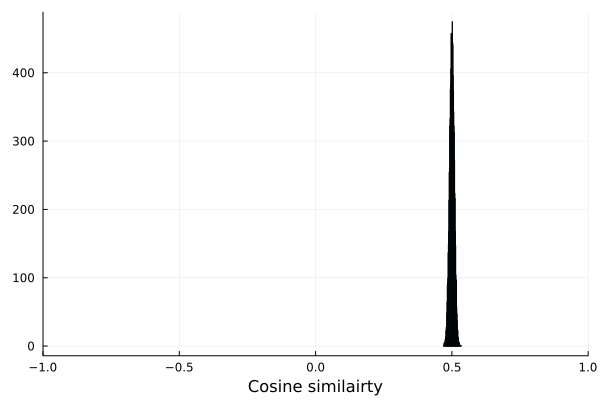
\includegraphics[scale = 0.7]{showcase}
    \caption{10000 cases of random 10000-dimensional bipolar vectors are made and each time implemented following example~\ref{eqn:ex1}. The resulting cosine similarities between $A$ and $A'$ are then plotted in a histogram.}
    \label{fig:exm1}
\end{figure}

We see that we can retrieve a lot of information with most of the cosine similarities centering around 0.5. Notice that two completely random HDVs would have a cosine similarity close to 0 just by stochastics. This result is not comparable to state-of-the-art accuracies but very efficient nonetheless as all of these calculations were done in less than 2 seconds. This same experiment was done with random binary 10000-dimensional vectors and it finished even faster as expected but retained the accuracy (similar \textit{Hamming distance} peak around 0.25).
\chapter[Hyperdimensional computing]{Hyperdimensional Computing}
Hyperdimensional computing (HDC) is a relatively recent paradigm of computing in which data is represented and manipulated by high-dimensional (or hyperdimensional) vectors in the range of tens of thousands bit. This framework, outlined by Kanerva~\cite{Kanerva2009}, is inspired by the workings of the human brain and its ability to adapt, learn fast and easily understand semantic relations. The human brain consists of about 100 billion neurons (nerve cells) and 1000 trillion synapses that connect these neurons. Each neuron is connected to up to 10,000 other neurons, creating massive circuits. This is likely fundamental to the workings of the human brain and what separates our brains from modern von Neumann computer architectures, which operate on 8 to 64-bit vectors. This becomes clear when we compare the relative simplicity for a human to learn a language compared to computers. Computers use a large and complicated set of arithmetic operations in the form of deep learning networks, which require terabytes of data and thousands of Watts of computing power to come close to mastering a language whilst a human can recognize other languages relatively easily when they don't even speak it. Likewise languages, we can very easily memorize and compare other intrinsically complex and contextual concepts such as images. A computer would have a hard time finding similarities between a set of images and faces because this requires very complex machine learning models. The human brain can do this all with a very large efficiency by consuming only roughly 20 W of energy.

Achieving these kinds of flexible brain-like models based on high dimensionality is not entirely new and is being explored since the 1990s. Some of these earlier models include Holographic Reduced Representations~\cite{HRR}, Spatter Code~\cite{spatter} and others. A hyperdimensional vector (HDV) can represent anything from a scalar number to any kind of concept. This vector is initially made up of totally random elements, but with a simple set of operations, which will be explained later, we can use other vectors to combine some concepts into new similar or dissimilar concepts. For example, to show the essence of HDC and how it tries to simulate the brain, we can compare the concept of a \textit{table} to the concept of a \textit{brocolli}. We would not immediately conclude that they are in any way similar but as humans, we can trace back \textit{table} to \textit{plate}, which has some similarities with \textit{food} from which we can easily extract the concept of \textit{brocolli} as in equation \ref{eqn:sem}. These kinds of operations are not very obvious for a classical computer but creating these semantic pathways and recognizing links between distant objects are rather easy for humans. Two unrelated concepts are noted by $\neq$ and two related concepts by $\approx$.
\begin{align}\label{eqn:sem}
    \begin{split}
    &\textrm{table} \neq \textrm{brocolli} \\        
    &\textrm{table} \approx \textrm{plate} \approx \textrm{food} \approx \textrm{brocolli}
    \end{split}
\end{align}
The elements in an HDV can be made up of binary bits (values from the set {0, 1}) like in classical computing but also of bipolar (values from the set {-1, 1}) or real numbers. The choice of the nature of the elements has also implications on the nature of the different operations and possibly the results.

An initial HDV is generated randomly. This \textit{holistic} or \textit{holographic} representation of a concept spread out over a vector consisting of thousands of bits gives rise to interesting properties such as its robustness agaisnt noise~\cite{hdctheo}. These kinds of systems are very tolerant to noise and failure of bits since we introduce a lot of redundancy in the vector just by stochastics. This is very unlike classical computing where every bit counts and one failure in a bit can lead to immediate data corruption. Besides its robustness, it also has the potential to perform much faster and more efficient computations than traditional computer systems since it allows for more efficient data storage by encoding multiple objects into a vector~\cite{Kanerva2009}\cite{hdctheo}.
\section{Operations on hyperdimensional vectors}
The interesting properties of HDC are based on only four basic operations we can perform on HDVs. We will discuss these for bipolar and binary vectors. From here, all implementations are written in the programming language Julia~\cite{Julia} unless noted otherwise. Known for its efficiency, Julia's blend of high-level, interpreter-based features makes it possible to write powerful programs. This is particularly beneficial when working with high-dimensional spaces. Julia's built-in support for bitvectors and bitmatrices, along with parallel computing, will be useful for this thesis. Furthermore, the lively Julia community supports a rich ecosystem and a broad array of packages to utilize.

Before the operations are demonstrated, we show how a random hyperdimensional vector can be generated in Julia. In the following code block, functions to generate binary and vectors can be made effortlessly with one line each.

\begin{minted}{julia}
# Built-in package for random number generation
using Random

# Binary HDV
bithdv(N::Int=10_000) = bitrand(N) 
#Bipolar HDV
hdv(N::Int=10_000) = rand((-1,1), N)
\end{minted}

\subsection*{Bundling} \label{sssec:add}
Also referred to as \textit{superposition} or \textit{aggregation}, the element-wise addition as in equation~\ref{eqn:sum} of $n$ input vectors $[X_{1} + X_{2} + \cdots + X_{n}]$ creates a vector $X$ that is similar to the input vectors.
\begin{equation}
    \label{eqn:sum}
    X = [X_{1} + X_{2} + \cdots + X_{n}]
\end{equation}
For bipolar vectors, this entails a straightforward element-wise addition. The resulting vector is restricted to a bipolar nature too depending on the sign of each element, thus containing only $-1$, $1$ but allowing $0$ for elements that are in disagreement as shown in the following $6$-dimensional example.
\begin{alignat*}{7}
    X_{1} &= && \qquad +1 && \qquad -1 && \qquad +1 && \qquad +1 && \qquad -1 && \qquad -1 \\
    X_{2} &= && \qquad +1 && \qquad +1 && \qquad +1 && \qquad -1 && \qquad -1 && \qquad -1 \\
    X_{3} &= && \qquad -1 && \qquad -1 && \qquad +1 && \qquad +1 && \qquad -1 && \qquad +1 \\
    X_{4} &= && \qquad -1 && \qquad -1 && \qquad -1 && \qquad +1 && \qquad -1 && \qquad +1 \\
    \hline
    [X_{1} + X_{2} + X_{3} + X_{4}] &= && \qquad \phantom{-}0 && \qquad -1 && \qquad +1 && \qquad +1 && \qquad -1 && \qquad \phantom{-}0
\end{alignat*}

For binary vectors, the vectors are element-wise bundled based on the majority element. This is no problem if an odd number of input vectors are considered but ambiguity rises when bundling an even set of vectors. This can be solved by setting the element in question randomly.~\cite{binBund} Another possibility is to add another random vector however this may seem to add more unnecessary noise, especially when bundling a low number of vectors. We can also reverse this by an \textit{inverse addition}. For bipolar vectors, this means just multiplying the vector of interest by -1. A binary vector can be flipped bit-wise. These kinds of operations are not directly built into Julia, but are easily programmed as followed:

\begin{minted}{julia}
# Adds bitvectors element-wise based on the majority element.
# Random if tied.
# Reduce function takes another function (here .+)
# and applies it to all given vectors.
# 'Dotted' operations such as .+ are vectorized
# making it element-wise.
function bitadd(vectors::BitVector ...)
    v = reduce(.+, vectors)            
    n = length(vectors) / 2
    x = [i > n ? 1 : i < n ? 0 : rand(Bool) for i in v]
    return x
end

# Adds bipolar vectors element-wise and rounds off to -1,0 or 1
# depending on the resulting sign.
add(vectors...) = reduce(.+, vectors) .|> sign
\end{minted}
Similar to an ordinary arithmetic summation, the bundling addition of hyperdimensional vectors is commutative so the result is not dependent on the order of addition.
\begin{equation}
    \label{eqn:sumcom}
    [X_{1} + X_{2}] = X = [X_{2} + X_{1}]
\end{equation}
\subsection*{Binding} \label{sssec:mult}
Two vectors can be multiplied element-wise resulting in a vector maximally dissimilar to the input vectors. Vectors $X$ and $Y$ are bound together forming $Z$ being orthogonal to $X$ and $Y$ as shown in equation~\ref{eqn:multp}.
\begin{equation}
    \label{eqn:multp}
    Z = X \circ Y
\end{equation}
This \textit{binding} operation translates to a simple arithmetic element-wise multiplication for bipolar vectors. For binary vectors, this is represented by a \textit{XOR} bit-operation shown as follows.
\begin{alignat*}{7}
    X &= && \qquad 1 && \qquad 0 && \qquad 1 && \qquad 1 && \qquad 0 && \qquad 0 \\
    Y &= && \qquad 1 && \qquad 1 && \qquad 0 && \qquad 1 && \qquad 0 && \qquad 1 \\
    \hline
    X \circ Y &= && \qquad 0 && \qquad 1 && \qquad 1 &&  \qquad 0 && \qquad 0 && \qquad 1
\end{alignat*}
In Julia, there is a built-in function to carry out bit-operations such as \textit{XOR}. For bipolar vectors, a simple element-wise multiplication suffices.

\begin{minted}{julia}
# Bind binary vectors
bitbind(vectors::BitVector ...) =  reduce(.xor, vectors)

# Bind bipolar vectors
bind(vectors...) = reduce(.*, vectors)
\end{minted}

The binding operation can also be undone by multiplying with the same vector again. It is its own inverse so that:
\begin{equation}
    \label{eqn:multpinv}
    A \circ A = O
\end{equation}
Where $O$ is a vector containing only zeros. Likewise an ordinary multiplication, this operation is commutative and distributive over additions, meaning that transforming a bundle of concepts with binding is equivalent to binding every element before bundling.
\begin{equation}
    \label{eqn:multpdis}
    A = Z \circ (X + Y) = X \circ Z + Y \circ\ Z
\end{equation}
\subsection*{Permutation} \label{sssec:perm}
The permutation operation of an HDV, is a reordering of the contents of the HDV. This can be random but a circular shift is widely employed~\cite{HD_rev} and makes the operation easily reversible. This results in a vector technically dissimilar from the input vector but still encoding its information. This will become important later when it will be used to encode sequential information such as tokens in a text. This operation will be denoted by $\Pi$.
\begin{alignat*}{7}
    X &= && \qquad 1 && \qquad 0 && \qquad 1 && \qquad 1 && \qquad 0 && \qquad 0 \\
    \hline
    \Pi(X) &= && \qquad 0 && \qquad 1 && \qquad 0 &&  \qquad 1 && \qquad 1 && \qquad 0
\end{alignat*}
In Julia, this line can do it for both binary and bipolar vectors:

\begin{minted}{julia}
# Permute by applying a circular shift
perm(vector::AbstractVector, k::Int=1) = circshift(vector, k)
\end{minted}

\subsection*{Similarity measurement} \label{sssec:sim}
For many kinds of problems, it will be necessary to quantify the similarity between two HDVs. The method depends on the nature of the vectors. For binary vectors, the \textit{Hamming distance} defined as:

\begin{equation}
    \label{eqn:Hamming}
    \text{Ham}(A, B) = \frac{1}{d} \sum_{i=1}^{d} 1_{A_{(i)} \neq B_{(i)}}
\end{equation}
The \textit{cosine distance} as defined in equation~\ref{eqn:cosine} is most commonly used for bipolar vectors:
\begin{equation}
    \label{eqn:cosine}
    cos(A, B) = \frac{A \cdot B}{||A|| * ||B||}
\end{equation}
Both are not built-in Julia by default, but can be programmed as followed:
\begin{minted}{julia}
# Built-in package for linear algebra operations 
using LinearAlgebra

# Hamming distance
hamming(x::BitVector, y::BitVector) = sum(x .!= y)/length(x)

# Cosine similarity
cosine(x::Vector, y::Vector) = dot(x, y) / (norm(x) * norm(y))
\end{minted}
The results of both of these measurements are summarized in table~\ref{tab:dist}.
\begin{table}[h]
    \centering
    \caption{\label{tab:dist}Overview of similarity measurements in HDC depending on the nature of the HDVs}
    \begin{tabular}{|cccc|}
        \hline
        \textbf{Measurement} & \textbf{Dissimilar} & \textbf{Orthogonal} & \textbf{Similar} \\
        \hline
        \textbf{Hamming distance} & 1 & 0.5 & 0 \\
        \hline
        \textbf{Cosine similarity} & -1 & 0 & 1 \\
        \hline
    \end{tabular} 
\end{table}

It is important to note that two random HDVs will be quasi-orthogonal to each other just by stochastics. Also notice that the first quantifies a distance and the latter a similarity.
\section{Examples}
There are many interesting possibilities given the relative simplicity of all these operations. In this section, we will demonstrate the power of hyperdimensional computing with some simple examples.
\subsection*{Simple example with simulated data}
To get a feel for the operations, assume $A, B, C, X, Y$ and $Z$ to be random 10,000-dimensional bipolar hypervectors and that $D = X \circ A + Y \circ B + Z \circ C$, let us then try to retrieve A from D by using the defined operations. We generate for $A, B, C, X, Y$ and $Z$ each a random 10,000-D vector. To retrieve an approximation of A, D can be multiplied by X and the rest of the included vectors are then regarded as noise as done in equations~\ref{eqn:ex1}. Because of the robustness of hyperdimensional vectors, a lot of information of A should still be contained within D.
\begin{align}\label{eqn:ex1}
\begin{split}
    A' &= X \circ D \\
    &= X \circ (X \circ A + Y \circ B + Z \circ C) \\
    &= \underbrace{X \circ X \circ A}_A + \underbrace{X \circ Y \circ B + X \circ Z \circ C}_\text{noise} \\
    &\approx A
\end{split}
\end{align}
 The procedure of equation~\ref{eqn:ex1} is repeated 10,000 times because of the stochastic nature of these vectors. The results are illustrated in figure~\ref{fig:exm1}.
\begin{figure}[h]
    \centering
    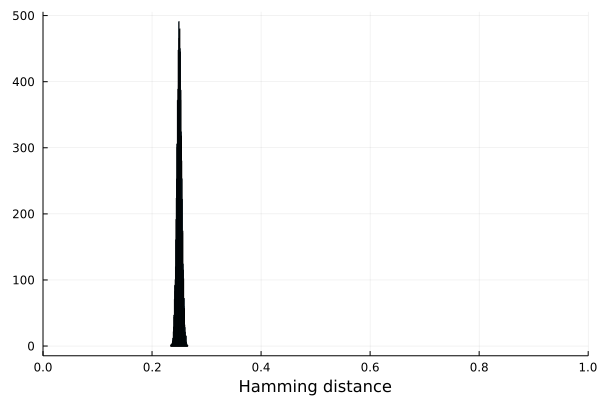
\includegraphics[scale = 0.2]{output.png}
    \caption{10,000 cases of random 10,000-dimensional binary vectors being made by equation~\ref{eqn:ex1}. The resulting Hamming distances between $A$ and $A'$ are then plotted in a histogram. Dashed line indicates a Hamming distance of 0.5, meaning that two vectors are orthogonal.}
    \label{fig:exm1}
\end{figure}
We see that we can retrieve a lot of information with most of the Hamming distances centering around 0.25. Due to the high-dimensional space and thus its robustness, the distances are very consistent. Notice that two completely random HDVs would have a distance close to 1 just by stochastics. A Hamming distance of 0 would mean that we retrieved all bits of A correctly, which is impossible in this model due to the consideration of noise. Although we work with a very constrained model, vector A is roughly 75 \% retrievable and the calculations are very efficient as all of these can be completed in less than 2 seconds on a laptop. This same experiment was done with random bipolar, 10,000-dimensional vectors and it performs slightly slower as expected but retained the accuracy.
\section{Examples of hyperdimensional computing with real datasets}
\label{sec:example}
Now, the power of these simple operations will be demonstrated by applying them to a couple of relatively small real datasets.
\subsection*{Zoo animal classification}
As the first example, we will consider a simple dataset containing 101 animals with 17 descriptors such as their number of legs, their skin covering and other physical properties~\cite{zoo}. Our goal is to create a simple model that can classify these animals and other animals that are not present in the dataset based on their descricptors. To tackle this problem, we first assign to each descriptor a random hyperdimensional vector. For each animal, all of its features can be bundled to obtain a final vector representing the animal. For example, it is known that a chicken lays eggs, is covered with feathers and has two legs so then these features can be bundled as in the following equation. $C$ is a vector representing a chicken, $E$ the ability to lay eggs, $F$ the possession of feathers and $T$ the possession two legs:
\begin{equation}\label{eqn:chicken}
    C = E + F + T
\end{equation}
This is simple for all the variables that have binary values, but the feature for the number of legs is variable. Although it is possible to assign completely random vectors to each number of legs, it would make a slightly more biologically realistic model if an animal with 2 legs would be more similar to one with 4 legs than to one with 8 legs. To address this, a range of numbers would have to be representable by hyperdimensional vectors, the range from 0 to 8 in this case. First, a random hyperdimensional vector representing the lower bound of the interval is generated. Next, a vector representing the next step in the interval is constructed by replacing a fraction of the vector with random bits. This last step is then repeated to obtain a vector of each number in a range.

In biology, it is possible to find higher-order of concepts that are combinations of directly observable characteristics. For example, an animal could lay eggs or be dependent on its mother's milk, but (almost) never both. So, the growth and development of an animal depend on these characteristics. This property can be easily implemented into this HDC model by binding an HDV of a higher order concept to the descriptor HDV. So as said previously, the 'milk' ($M$), and 'egg' ($E$) features yields information about the growth of the animal, so we will create another vector representing the growth feature ($G$) to obtain a more expanded model. This is also done for the skin protection features ($S$) and all the features considering the limbs ($L$). This also gives us the possibility to retrieve some features of the animals as in the procedure shown in the previous example. Thus, equation~\ref{eqn:chicken} can be expanded into:
\begin{equation}
    C = G \circ E + S \circ F + L \circ T
\end{equation}

After conducting the various procedures, the data set now consists of 101 animals, each represented by a 10,000-dimensional feature vector. To efficiently analyze and visualize this high-dimensional data, principal component analysis (PCA) has been employed to reduce the dimensionality from 10,000 to just two. By projecting these vectors onto a 2D space, the data can be conveniently displayed in a two-dimensional plot, as illustrated in Figure \ref{fig:exm2}. Upon examination of the plot, three distinct and meaningful clusters of animal classes emerge, which align well with our understanding of evolutionary relationships. These clusters include: (1) mammals, (2) a group consisting of birds, reptiles, and amphibians, and (3) a cluster encompassing invertebrates and insects. While the current analysis already provides valuable insights into the relationships between different animal classes, further improvement could be achieved by incorporating additional features that may lead to a clearer separation of these groups. By doing so, the model would be able to more accurately distinguish between the different animal classes and provide a more comprehensive understanding of their evolutionary connections.
\begin{figure}[h]
    \centering
    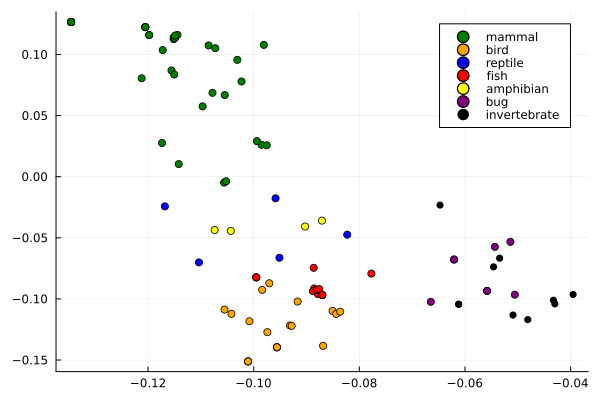
\includegraphics[scale = 0.5]{pca1.png}
    \caption{Scatter-plot of the first two principal components (PCs) of a 101$\times$10,000 matrix containing hyperdimensional vectors for every animal in the zoo dataset after a PCA procedure. These PCs account for roughly 48 \% of the variance.}
    \label{fig:exm2}
\end{figure}

After an HDV has been made for every animal, all animals of the same class can be bundled to obtain an HDV representing the said class. So for example, if we have a hyperdimensional vector for a pigeon ($P$), chicken ($C$) and a kiwi ($K$), an HDV representing birds ($B$) can be made by doing:
\begin{equation}
    B = [P + C + K]
\end{equation} 
To classify an animal, its HDV can be compared to the HDVs of every class and the most similar vector is then assumed to be its class.  In the following code block, the hypervectors for every animal and class have been already made as discussed above. The resulting HDV for a flamingo has been compared to every other class vector \textit{via} a measurement of the Hamming distance. The distance of flamingo HDV to the bird HDV is significantly smaller than to all other vectors
\begin{figure}[H]
    \centering
\begin{minted}{julia}
# HDVs for every animal class HDVs have been made already
# Take flamingo HDV out of dataframe
flamingo = data.species_hdv[24]
println("Hamming distance to mammal = ",
hamming(flamingo, mammal))

println("Hamming distance to bird = ",
hamming(flamingo, bird))

println("Hamming distance to reptile = ",
hamming(flamingo, reptile))

println("Hamming distance to amphibian = ",
hamming(flamingo, amphibian))

println("Hamming distance to bug = ",
hamming(flamingo, bug))

println("Hamming distance to fish = ",
hamming(flamingo, fish))

println("Hamming distance to invertebrate = ",
hamming(flamingo, invertebrate))

# Output
# Hamming distance to mammal = 0.303
# Hamming distance to bird = 0.1044
# Hamming distance to reptile = 0.2727
# Hamming distance to amphibian = 0.313
# Hamming distance to bug = 0.2867
# Hamming distance to fish = 0.3484
# Hamming distance to invertebrate = 0.4061
\end{minted}
\end{figure}
For further improvement, it would be possible to generate a set of animals not present in the dataset and test those in order to further understand how this model can be improved. On top of this, it would also be possible to generate a confusion matrix to understand where we could use more distinguishing descriptors. From the PCA, we could already predict that reptiles and amphibians would be easily confused, as for invertebrates and bugs.
\subsection*{Protein classification}
\label{ssec:protclas}
To illustrate an example more akin to this research topic, a model based on the principles of hyperdimensional computing will be built to classify a protein sequence dataset~\cite{anticancer}. It contains 949 manually curated peptide sequences with their membranolytic anti-breast cancer activity level (very active, moderately active, experimentally inactive and virtually inactive). The virtually inactive peptides are predicted to be inactive. The model will be built with mostly the same procedure as for the animal classifier, but instead of animals, sequences have to be encoded into HDVs now. First, a random HDV is generated for every amino acid. Physicochemical properties, evolutionary constraints etc. could be introduced to make this model more realistic but that is not necessary for this demonstration. Next, a peptide sequence is to be considered as a bag of trimers as seen in figure~\ref{fig:diagram_exprot5}. A vector representing a trimer is generated by binding the three amino acids whilst retaining sequential information by shifting as in equation~\ref{eqn:trimer}. All retrievable trimers from a given sequence are then bundled together, forming a vector representative of the sequence. 
\begin{equation}\label{eqn:trimer}
    ABC = A \circ \Pi (B) \circ \Pi (\Pi (C))
\end{equation}
\begin{figure}[h]
    \centering
    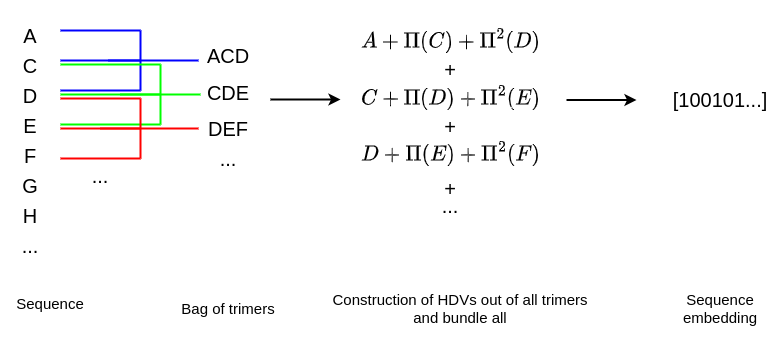
\includegraphics[scale = 0.55]{diagram_exprot.png}
    \caption{Overview of operations done to obtain an HDV of a protein sequence for the example concerning the real peptide dataset. First, a random HDV is generated for every amino acid. Next, a peptide sequence is to be considered as a bag of trimers. A vector representing a trimer is generated by binding the three amino acids whilst retaining sequential information by shifting as in equation~\ref{eqn:trimer}. All retrievable trimers from a given sequence are then bundled together, forming a hyperdimensional vector representation of the sequence.}
    \label{fig:diagram_exprot5}
\end{figure}
From here on, the same procedures as in the last example can be applied here too, so all HDVs of a class are bundled for further analysis. The PCA procedure did not generate interesting results because the two first principal components explained only 5 \% of the variance. This means that it is not feasible to reduce the 10,000 dimensions of the vectors to two, likely because the information is too smeared out over the vectors. This occurrence is highly dependent on the training data. Nevertheless, this follows the philosophy of hyperdimensional computing in keeping holistic representations of concepts.

\begin{figure}[H]
    \centering
    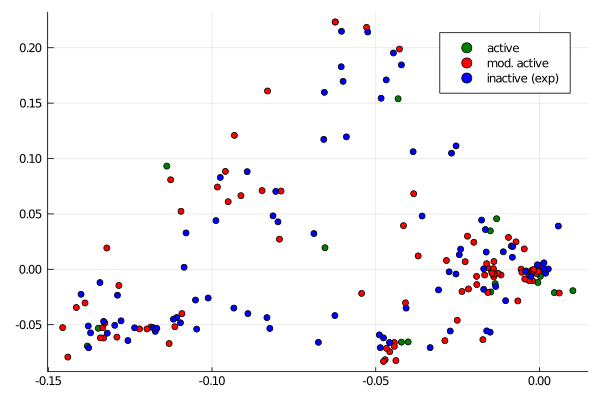
\includegraphics[scale = 0.5]{exampprot.png}
    \caption{Scatter-plot of the first two principal components, projecting the 10,000-dimensional vectors for every peptide into the 2 main PCs. These PCs account for roughly 5 \% of the total variance}
    \label{fig:diagram_exprot}
\end{figure}

Next, a classifier was made correspondingly. The dataset was stratified and split into a training set (comprising 80 \% of the sequences) and a test set. With 100 runs, it could predict a protein sequence's class with an accuracy of 85 \%. It has to be taken into account that the predicted inactive peptides account for 80 \% of the sequences of the dataset, thus this model performs slightly better than if we would predict at random. There are many possible improvements to be made however, such as using more suitable performance metrics, introducing similarities between amino acids instead of setting them randomly and using more suitable frameworks for our protein classification models, which will all be research topics further on in this project.
\input{chapt_perf_embd}
\chapter{Case study:\\PhaLP dataset}
To implement and evaluate hyperdimensional computing in real-life problems, the potential of hyperdimensional computing will be evaluated on the PhaLP dataset~\cite{phalp} for this chapter. PhaLP is a comprehensive database currently comprising more than 17000 entries of phage lytic proteins including much of their information such as their type, domains and tertiary structures. Phage lytic proteins are used by bacteriophages to infect bacterial cells. To cross the bacterial cell walls, phages use two different types of phage lytic proteins: virion-associated lysins (VALs) and endolysins. Phage lytic proteins also comprise one or more functional domains categorized into two classes: enzymatically active domains (EADs) and cell wall binding domains (CBDs).

All 17356 unique protein sequences were embedded into hyperdimensional vectors. This took only a few minutes for every method on a consumer laptop.

\section{Type classifcation}
Only a fraction of the database is manually annotated to include the protein's type because the amount of phage lytic proteins whose type is described in the literature is relatively small. The developers of PhaLP resorted to a machine learning approach for the classification of unannotated sequences. They embedded each protein sequence \textit{via} SeqVec~\cite{seqvec} and trained a random forest classifier with 100 estimators and balanced weights to classify the proteins whose types were unknown. For this case study, we attempted to simulate their experiments of classifying the proteins into types based on their sequence using several methods. As of March 2023, the latest version of the PhaLP database,~\textit{v2021\_04}, has been used to test our models.
\subsection*{Embedding of sequences into hyperdimensional vectors}
First, we used several sequence encoding techniques tested on several kinds of base vectors. In chapter~\ref{ssec:protclas}, a method of embedding sequences of amino acids has already been discussed. Here, a sequence of amino acids is considered to be a bag of k-mers. Within a k-mer, the amino acids (presented as randomly generated hyperdimensional vectors) are bonded together with sequential information included. All possible k-mers are all then bundled together, the result is then a hyperdimensional vector representing the whole sequence. We also introduce a novel sequence embedding method within the framework of hyperdimensional computing. It is similar to the bag-of-words method in the sense that it bundles vectors of k-mers, but here, the k-mer's positional information will be encoded into the k-mer before bundling. Insert figure The resulting sequences are then visually assessed \textit{via} PCA.

There was no visual difference between the PCA plots for the bag-of-words method and the convolutional method, but there is a clear difference between the different starting embeddings. The sequence embeddings from both the bag-of-words method and the convolutional method made with ESM AA embeddings seem to capture more of the variance between the sequences. To demonstrate hyperdimensional computing as an option for machine learning applications, several methods using this framework have been developed and tested. Out of the 11549 unambiguous UniParc accessions in the newest version of the database, 4829 are manually annotated on their type. Out of these manually annotated proteins, 2803 are endolysins and 2026 are VALs.

\begin{figure}[H]
    \centering
    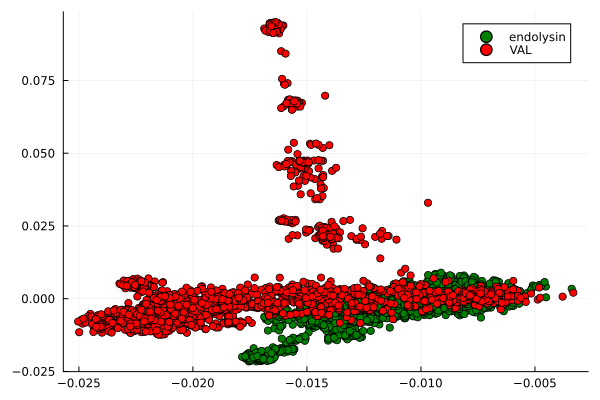
\includegraphics[scale = 0.5]{phalp_bow_rand}
    \caption{Scatter-plot of the first two principal components of the encoded phage lytic proteins. The sequences were encoded via the bag-of-words method starting from random hyperdimensional vectors. Only manually annotated phage lytic proteins were considered and are color-coded based on their type. These PCs account for roughly 7 \% of the total variance in the system.}
    \label{fig:phalpbowrand}
\end{figure}

\begin{figure}[H]
    \centering
    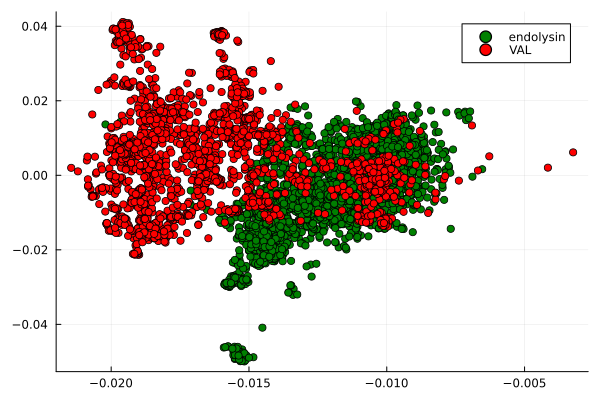
\includegraphics[scale = 0.5]{phalp_bow_esm}
    \caption{Scatter-plot of the first two principal components the encoded phage lytic protein. The sequences were encoded via the bag-of-words method starting from hyperdimensionally-extended ESM embeddings. Only manually annotated phage lytic proteins were considered and are color-coded based on their type. These PCs account for roughly 15.5 \% of the total variance in the system.}
    \label{fig:phalpbowesm}
\end{figure}

\subsection*{Naive hyperdimensional addition}\label{ssec:purehdc}
As a baseline level, we use the rudimentary HDV classification technique as seen in chapter~\ref{sec:example}: the HDVs of sequences of the same class are bundled to construct single HDVs representative of every class. Then, a sequence's class is inferred by comparing the sequence's HDV to both class HDV \textit{via} a similarity measure based on the assumption that the class vector is maximally similar to its components. This model was evaluated \textit{via} a stratified 10-fold cross validation.
\begin{table}[h]
    \caption{\label{tab:phalpclass}Results of type classifications using the principal classification technique of hyperdimensional computing and an XGBoost classifier with several kinds of embeddings}
    \resizebox{\textwidth}{!}{\begin{tabular}{|c||c|c|c|c|}
        \hline
        \underline{F1-scores} & \textbf{BoW/random} & \textbf{BoW/ESM} & \textbf{Convolutional/random} & \textbf{Convolutional/ESM} \\
        \hline
        \textbf{Naive addition} & 0.1458 & 0.1468 & 0.1461 & 0.1461 \\
        \hline
        \textbf{XGBoost classifier} & 0.9667 & 0.9754 & 0.9661 & 0.986 \\
        \hline
    \end{tabular}}
\end{table}

It is feasible to learn the classes of every sequence using only operations within the hyperdimensional computing framework. This is done by using the same techniques as in chapter~\ref{sec:example}. Evaluating our model using stratified 10-fold cross-validation results in F1-scores of around 0.14 for every kind of hyperdimensional embedding. This low result is likely due to the possibility of oversaturation of the class vectors.

We can predict the angle between a class vector and a randomly selected vector from said class by $\Theta = \arccos({2k \choose k}/2^{2k})$ with $2k+1$ equal to the number of sequences in the class~\cite{sathdv}. This approximation is valid for bipolar vectors in hyperdimensions $(\ge 10000)$. This equation also suggests that an increase in dimensions will not influence the angle. Evaluating this equation by considering random 1001 vectors in a class, so $k = 500$, results in an angle of $88.6^{\circ}$. This indicates that a vector has a limited capacity: the more vectors we bundle together, the closer the angle will be to $90^{\circ}$ and thus the more dissimilar the class vector becomes to its components. This results in the class vectors not being representative anymore of a given dataset. This equation assumes that the class vector is a bundle of purely random vectors which is not the case for our embeddings; however, it provides us a rough idea about the bundling capacity of a hyperdimensional vector. Thus, using the rudimentary model works only for very small datasets, as seen in the examples in chapter~\ref{sec:example}. So to encode larger datasets, the training algorithm has to be more refined.

\subsection*{Machine learning models with binary hyperdimensional embeddings}
The baseline hyperdimensional classification model has been compared to a more established model, the XGBoost classifier. The classification with an XGBoost classifier is done via the default XGBoost classifier from \textit{XGBoost.jl v2.2.5} and is evaluated \textit{via} \textit{MLJ.jl v0.19.5} with also a stratified 10-fold cross validation. The results with this model for every embedding (provided in table~\ref{tab:phalpclass}) are much more comparable to the results of the experiment in the PhaLP paper. This is an indication that hyperdimensional computing can provide a very fast and reliable method of embedding protein sequences, even without prior biological information. 

The drawback of this machine learning model, which is to be expected from every gradient-based model, is that training and predictions take much longer to compute compared to hyperdimensional training models. The cross validation procedure took up to 5 minutes on a consumer-grade laptop, whilst with the naive additive approach, the procedure took less than 10 seconds to finish.

\subsection*{OnlineHD implementation}
As an answer for the unsatisfactory results of the rudimentary additive approach in part~\ref{ssec:purehdc}, another hyperdimensional computing approach has been assessed for our use case. OnlineHD by A. Hernandez-Cano~\textit{et al.}~\cite{onlinehd} is an algorithm that expands on the classical hyperdimensional training methods by trying to eliminate model saturation. Instead of naively bundling vectors on top of each other, this algorithm assigns weights to every addition  depending on how much new information it adds to the model to prevent class vector saturation.

To train the model, assume a new data point $\vec{V}$ with label $l$ and class vectors $\vec{C_{i}}$ with each having a label $i$. The cosine similarity of $\vec{V}$ with every class vector is then calculated as $cos_{i}$. If $\vec{V}$ with an actual label $l$ would have been predicted as $l'$, the class vectors will be updated as followed (with learning rate $\eta$):

\begin{alignat}{1}
    \label{eqn:onlinehd}
    \vec{C_{l}} &\leftarrow \vec{C_{l}} + \eta (1 - cos_{l}) * \vec{V} \\
    \vec{C_{l'}} &\leftarrow \vec{C_{l'}} - \eta (1 - cos_{l'}) * \vec{V}
\end{alignat}

This means that if a new data point is highly dissimilar to its class vector and thus contains a high amount of new information, the weight of the update will increase. The information is then also subtracted from the incorrectly predicted class vector. If a label would be correctly predicted for a new data point, the model will not be updated to avoid saturation. To initialize the model, the first vector of a class to be assessed is assumed to be the class vector. Due to the nature of this model, we cannot constrict our hyperdimensional embeddings to a bipolar or binary nature anymore and the embeddings are then allowed to be real-numbered. Mathematical operations such as multiplications and additions are then assumed to be element-wise.

On top of single-pass model as discussed above, A. Hernandez-Cano~\textit{et al.} also implemented an iterative retraining algorithm to increase the accuracy of OnlineHD. This starts from the class vectors made \textit{via} the single-pass OnlineHD model, but assesses the class vectors by performing inference with every training vector. If a training vector's label is wrongly predicted, equations 4.1 and 4.2 are then used to update the model. This all is then iterated for a given amount of cycles.

To test these algorithms, real-numbered embeddings have to be made from our subject sequences. The same bag-of-words and convolutional approaches as well as the random and ESM base vectors are also applied here, but all starting from random vectors with values in $[-1, 1]$. These embeddings were assessed \textit{via} a scatter-plot of the two first principal components of their PCA projection. (insert firgures)

Since these algorithms are only available as PyTorch implementations, implementations in Julia have been made here. A stratified 10-fold cross validation of these models with our subject sequences has been performed. The learning rate is set at 0.035 and the amount of retraining iterations is set to 120. The results are provided in table~\ref{tab:phalpclassonline}. At first, there is generally a substantial increase in the performance of this model compared to the naive additive model. The single-pass model seems to have widely varying results depending on the type of embeddings used, with the bag-of-words embeddings generally performing better than the convolutional embeddings and also the ESM-based embeddings performing better than random base vectors. Iterative retraining of the model also seems to increase its performance significantly, even coming close to the performance of an XGBoost classifier in this case. Further improvement might be found when optimizing the models' parameters.

The cross validation procedure takes less than 10 seconds to run for the single-pass model, whilst doing a retraining of the model adds 2 to 3 minutes. This model appears to be a decently performing extension of the rudimentary hyperdimensional classification model for protein language modeling, whilst still being much more efficient than the commonly used machine learning models. The drawback of the model is that we cannot use hyperefficient bit-operations anymore, which limits its efficiency compared to the binary nature of the additive model.

\begin{table}[h]
    \caption{\label{tab:phalpclassonline}Results of type classifications using implementations of OnlineHD with several kinds of embeddings}
    \resizebox{\textwidth}{!}{\begin{tabular}{|c||c|c|c|c|}
        \hline
        \underline{F1-scores} & \textbf{BoW/random} & \textbf{BoW/ESM} & \textbf{Convolutional/random} & \textbf{Convolutional/ESM} \\
        \hline
        \textbf{Single-pass OnlineHD} & 0.8901 & 0.9214 & 0.7793 & 0.8400 \\
        \hline
        \textbf{Iterative OnlineHD} & 0.9487 & 0.9757 & 0.9486 & 0.9670 \\
        \hline
    \end{tabular}}
\end{table}

\section{Domain classification}
possible domain classification implementation, may or may not be interesting, but would be again a sequence classification (bit more complex perhaps) that we already tackled 
% ------------ REFERENCES ------------
% Here you have your bibliography created
\addcontentsline{toc}{chapter}{Bibliography} %show bibliography in TOC
\bibliographystyle{unsrt}  %apalike,phdbib.bst
\bibliography{Thesis_bib}
% Here you insert your appendices
\appendix
\begin{appendices}

% Dit voegt het woord Bijlage toe aan de titel!
\titleformat{\chapter} % command
  [display] % shape
  {\fontsize{18}{22} \selectfont \coltitle } % format
  {\MakeUppercase{\chaptertitlename \ \thechapter}} % the label
  {-2ex} %separator space
  {\fontsize{24}{32} \selectfont \bf \raggedright \MakeUppercase{\uline{#1}}} %before code
  { } %aft%after code


\chapter{Additional information on Chapter 3}\label{app:chp3}
\begin{figure}[h!]
    \centering
    \begin{subfigure}{0.48\textwidth}
        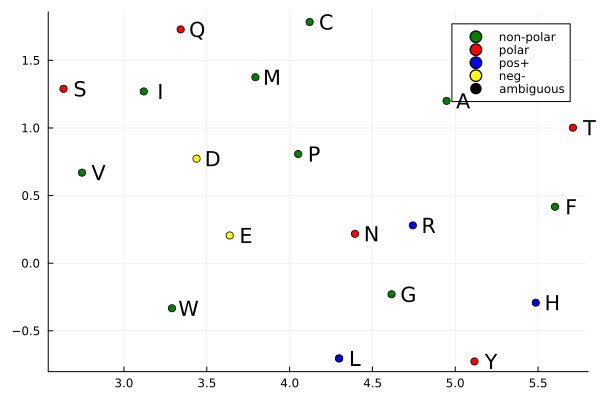
\includegraphics[width=\textwidth]{ur4tr_emb}
        \caption{Made starting from random hyperdimensional vectors for each amino acid, $k=4$.}
        \label{fig:AAtr4ru}
    \end{subfigure}
    \hfill
    \begin{subfigure}{0.48\textwidth}
        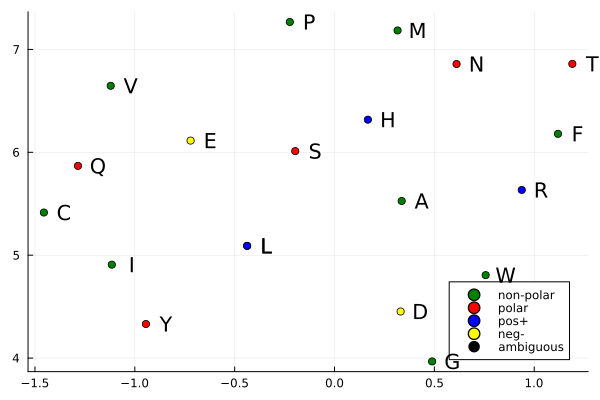
\includegraphics[width=\textwidth]{ur50tr_emb}
        \caption{Made starting from random hyperdimensional vectors for each amino acid, $k=50$.}
        \label{fig:AAtr50ru}
    \end{subfigure}
    
    \begin{subfigure}{0.48\textwidth}
        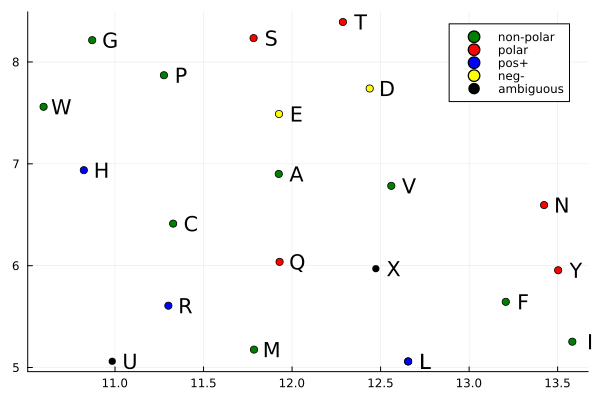
\includegraphics[width=\textwidth]{u4tr_emb}
        \caption{Made starting from extended ESM-2 embeddings for each amino acid, $k=4$.}
        \label{fig:AAtr4u}
    \end{subfigure}
    \hfill
    \begin{subfigure}{0.48\textwidth}
        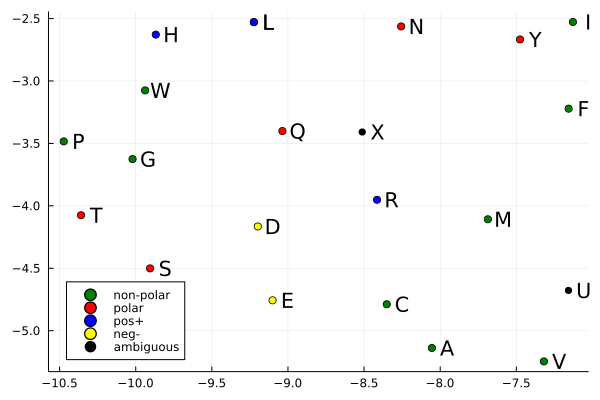
\includegraphics[width=\textwidth]{u50tr_emb}
        \caption{Made starting from extended ESM-2 embeddings for each amino acid, $k=50$.}
        \label{fig:AAtr50u}
    \end{subfigure}
    \caption{Scatter plot of a two-dimensional UMAP projection of the average amino acid HDVs with neighborhood-information of $k$ encoded. Learned from the human reference proteome. The amino acids are annotated and colored based on their chemical property of polarity.}
    \label{fig:main3}
\end{figure}

\begin{table}[h!]
    \label{tbl:target_grant}
    \caption{Target similarities made from Grantham's distance matrix}
    \resizebox{\textwidth}{!}{\begin{tabular}{cccccccccccccccccccc}
        $0.0$ & $0.73$ & $0.87$ & $0.8$ & $0.87$ & $0.73$ & $0.87$ & $0.8$ & $0.8$ & $0.8$ & $0.8$ & $0.87$ & $0.8$ & $0.8$ & $0.8$ & $0.67$ & $0.73$ & $0.73$ & $0.93$ & $0.87$\\ \hline
        $0.73$ & $0.0$ & $0.93$ & $1.0$ & $0.87$ & $0.93$ & $0.93$ & $0.8$ & $0.93$ & $0.8$ & $0.8$ & $0.93$ & $0.93$ & $0.93$ & $0.93$ & $0.8$ & $0.8$ & $0.8$ & $0.87$ & $0.87$\\ \hline
        $0.87$ & $0.93$ & $0.0$ & $0.6$ & $0.93$ & $0.8$ & $0.8$ & $0.93$ & $0.8$ & $1.0$ & $0.93$ & $0.67$ & $0.8$ & $0.73$ & $0.87$ & $0.73$ & $0.8$ & $0.93$ & $1.0$ & $0.93$\\ \hline
        $0.8$ & $1.0$ & $0.6$ & $0.0$ & $0.93$ & $0.87$ & $0.73$ & $0.93$ & $0.67$ & $0.93$ & $0.87$ & $0.73$ & $0.8$ & $0.6$ & $0.73$ & $0.73$ & $0.8$ & $0.87$ & $0.93$ & $0.87$\\ \hline
        $0.87$ & $0.87$ & $0.93$ & $0.93$ & $0.0$ & $0.93$ & $0.8$ & $0.73$ & $0.93$ & $0.73$ & $0.73$ & $0.93$ & $1.0$ & $0.93$ & $0.93$ & $0.87$ & $0.87$ & $0.8$ & $0.67$ & $0.53$\\ \hline
        $0.73$ & $0.93$ & $0.8$ & $0.87$ & $0.93$ & $0.0$ & $0.87$ & $1.0$ & $0.87$ & $1.0$ & $0.93$ & $0.73$ & $0.87$ & $0.87$ & $0.87$ & $0.73$ & $0.87$ & $0.93$ & $0.87$ & $0.93$\\ \hline
        $0.87$ & $0.93$ & $0.8$ & $0.73$ & $0.8$ & $0.87$ & $0.0$ & $0.93$ & $0.8$ & $0.93$ & $0.87$ & $0.67$ & $0.87$ & $0.73$ & $0.73$ & $0.8$ & $0.87$ & $0.93$ & $0.87$ & $0.6$\\ \hline
        $0.8$ & $0.8$ & $0.93$ & $0.93$ & $0.73$ & $1.0$ & $0.93$ & $0.0$ & $0.93$ & $0.6$ & $0.67$ & $0.93$ & $0.93$ & $0.93$ & $0.93$ & $0.87$ & $0.8$ & $0.53$ & $0.93$ & $0.8$\\ \hline
        $0.8$ & $0.93$ & $0.8$ & $0.67$ & $0.93$ & $0.87$ & $0.8$ & $0.93$ & $0.0$ & $0.87$ & $0.8$ & $0.73$ & $0.8$ & $0.67$ & $0.6$ & $0.73$ & $0.8$ & $0.87$ & $0.93$ & $0.87$\\ \hline
        $0.8$ & $0.8$ & $1.0$ & $0.93$ & $0.73$ & $1.0$ & $0.93$ & $0.6$ & $0.87$ & $0.0$ & $0.6$ & $0.93$ & $0.93$ & $0.87$ & $0.87$ & $0.87$ & $0.8$ & $0.67$ & $0.87$ & $0.8$\\ \hline
        $0.8$ & $0.8$ & $0.93$ & $0.87$ & $0.73$ & $0.93$ & $0.87$ & $0.67$ & $0.8$ & $0.6$ & $0.0$ & $0.87$ & $0.87$ & $0.73$ & $0.8$ & $0.8$ & $0.8$ & $0.67$ & $0.8$ & $0.8$\\ \hline
        $0.87$ & $0.93$ & $0.67$ & $0.73$ & $0.93$ & $0.73$ & $0.67$ & $0.93$ & $0.73$ & $0.93$ & $0.87$ & $0.0$ & $0.87$ & $0.73$ & $0.73$ & $0.67$ & $0.73$ & $0.93$ & $1.0$ & $0.87$\\ \hline
        $0.8$ & $0.93$ & $0.8$ & $0.8$ & $1.0$ & $0.87$ & $0.87$ & $0.93$ & $0.8$ & $0.93$ & $0.87$ & $0.87$ & $0.0$ & $0.8$ & $0.87$ & $0.8$ & $0.8$ & $0.87$ & $1.0$ & $0.93$\\ \hline
        $0.8$ & $0.93$ & $0.73$ & $0.6$ & $0.93$ & $0.87$ & $0.73$ & $0.93$ & $0.67$ & $0.87$ & $0.73$ & $0.73$ & $0.8$ & $0.0$ & $0.67$ & $0.73$ & $0.8$ & $0.87$ & $0.87$ & $0.8$\\ \hline
        $0.8$ & $0.93$ & $0.87$ & $0.73$ & $0.93$ & $0.87$ & $0.73$ & $0.93$ & $0.6$ & $0.87$ & $0.8$ & $0.73$ & $0.87$ & $0.67$ & $0.0$ & $0.8$ & $0.8$ & $0.93$ & $0.93$ & $0.87$\\ \hline
        $0.67$ & $0.8$ & $0.73$ & $0.73$ & $0.87$ & $0.73$ & $0.8$ & $0.87$ & $0.73$ & $0.87$ & $0.8$ & $0.67$ & $0.8$ & $0.73$ & $0.8$ & $0.0$ & $0.67$ & $0.87$ & $0.93$ & $0.87$\\ \hline
        $0.73$ & $0.8$ & $0.8$ & $0.8$ & $0.87$ & $0.87$ & $0.87$ & $0.8$ & $0.8$ & $0.8$ & $0.8$ & $0.73$ & $0.8$ & $0.8$ & $0.8$ & $0.67$ & $0.0$ & $0.73$ & $0.87$ & $0.87$\\ \hline
        $0.73$ & $0.8$ & $0.93$ & $0.87$ & $0.8$ & $0.93$ & $0.93$ & $0.53$ & $0.87$ & $0.67$ & $0.67$ & $0.93$ & $0.87$ & $0.87$ & $0.93$ & $0.87$ & $0.73$ & $0.0$ & $0.93$ & $0.8$\\ \hline
        $0.93$ & $0.87$ & $1.0$ & $0.93$ & $0.67$ & $0.87$ & $0.87$ & $0.93$ & $0.93$ & $0.87$ & $0.8$ & $1.0$ & $1.0$ & $0.87$ & $0.93$ & $0.93$ & $0.87$ & $0.93$ & $0.0$ & $0.6$\\ \hline
        $0.87$ & $0.87$ & $0.93$ & $0.87$ & $0.53$ & $0.93$ & $0.6$ & $0.8$ & $0.87$ & $0.8$ & $0.8$ & $0.87$ & $0.93$ & $0.8$ & $0.87$ & $0.87$ & $0.87$ & $0.8$ & $0.6$ & $0.0$
        \end{tabular}}
\end{table}

\begin{table}[h!]
    \label{tbl:achieved_grant}
    \caption{Achieved similarities targeting Grantham's distance matrix}
    \resizebox{\textwidth}{!}{\begin{tabular}{cccccccccccccccccccc}
        $0.0$ & $0.49$ & $0.49$ & $0.48$ & $0.48$ & $0.49$ & $0.5$ & $0.49$ & $0.49$ & $0.5$ & $0.49$ & $0.49$ & $0.49$ & $0.49$ & $0.49$ & $0.48$ & $0.5$ & $0.51$ & $0.49$ & $0.49$\\ \hline
$0.49$ & $0.0$ & $0.49$ & $0.5$ & $0.49$ & $0.49$ & $0.49$ & $0.5$ & $0.5$ & $0.48$ & $0.5$ & $0.5$ & $0.5$ & $0.49$ & $0.48$ & $0.49$ & $0.49$ & $0.49$ & $0.49$ & $0.49$\\ \hline
$0.49$ & $0.49$ & $0.0$ & $0.49$ & $0.49$ & $0.49$ & $0.49$ & $0.49$ & $0.49$ & $0.5$ & $0.49$ & $0.49$ & $0.5$ & $0.49$ & $0.49$ & $0.5$ & $0.49$ & $0.5$ & $0.49$ & $0.49$\\ \hline
$0.48$ & $0.5$ & $0.49$ & $0.0$ & $0.49$ & $0.48$ & $0.5$ & $0.5$ & $0.49$ & $0.49$ & $0.49$ & $0.5$ & $0.5$ & $0.5$ & $0.49$ & $0.5$ & $0.49$ & $0.49$ & $0.49$ & $0.49$\\ \hline
$0.48$ & $0.49$ & $0.49$ & $0.49$ & $0.0$ & $0.5$ & $0.5$ & $0.5$ & $0.49$ & $0.49$ & $0.5$ & $0.5$ & $0.5$ & $0.49$ & $0.5$ & $0.5$ & $0.51$ & $0.51$ & $0.5$ & $0.49$\\ \hline
$0.49$ & $0.49$ & $0.49$ & $0.48$ & $0.5$ & $0.0$ & $0.5$ & $0.49$ & $0.5$ & $0.49$ & $0.49$ & $0.5$ & $0.49$ & $0.49$ & $0.49$ & $0.5$ & $0.5$ & $0.49$ & $0.5$ & $0.5$\\ \hline
$0.5$ & $0.49$ & $0.49$ & $0.5$ & $0.5$ & $0.5$ & $0.0$ & $0.5$ & $0.51$ & $0.5$ & $0.5$ & $0.5$ & $0.5$ & $0.49$ & $0.49$ & $0.49$ & $0.49$ & $0.5$ & $0.48$ & $0.49$\\ \hline
$0.49$ & $0.5$ & $0.49$ & $0.5$ & $0.5$ & $0.49$ & $0.5$ & $0.0$ & $0.48$ & $0.49$ & $0.49$ & $0.51$ & $0.5$ & $0.5$ & $0.49$ & $0.5$ & $0.49$ & $0.5$ & $0.5$ & $0.5$\\ \hline
$0.49$ & $0.5$ & $0.49$ & $0.49$ & $0.49$ & $0.5$ & $0.51$ & $0.48$ & $0.0$ & $0.5$ & $0.49$ & $0.5$ & $0.5$ & $0.49$ & $0.5$ & $0.5$ & $0.48$ & $0.49$ & $0.49$ & $0.49$\\ \hline
$0.5$ & $0.48$ & $0.5$ & $0.49$ & $0.49$ & $0.49$ & $0.5$ & $0.49$ & $0.5$ & $0.0$ & $0.5$ & $0.5$ & $0.49$ & $0.49$ & $0.49$ & $0.49$ & $0.49$ & $0.5$ & $0.5$ & $0.48$\\ \hline
$0.49$ & $0.5$ & $0.49$ & $0.49$ & $0.5$ & $0.49$ & $0.5$ & $0.49$ & $0.49$ & $0.5$ & $0.0$ & $0.49$ & $0.49$ & $0.51$ & $0.5$ & $0.49$ & $0.5$ & $0.5$ & $0.49$ & $0.49$\\ \hline
$0.49$ & $0.5$ & $0.49$ & $0.5$ & $0.5$ & $0.5$ & $0.5$ & $0.51$ & $0.5$ & $0.5$ & $0.49$ & $0.0$ & $0.5$ & $0.49$ & $0.5$ & $0.49$ & $0.5$ & $0.49$ & $0.5$ & $0.49$\\ \hline
$0.49$ & $0.5$ & $0.5$ & $0.5$ & $0.5$ & $0.49$ & $0.5$ & $0.5$ & $0.5$ & $0.49$ & $0.49$ & $0.5$ & $0.0$ & $0.49$ & $0.5$ & $0.49$ & $0.5$ & $0.49$ & $0.5$ & $0.48$\\ \hline
$0.49$ & $0.49$ & $0.49$ & $0.5$ & $0.49$ & $0.49$ & $0.49$ & $0.5$ & $0.49$ & $0.49$ & $0.51$ & $0.49$ & $0.49$ & $0.0$ & $0.49$ & $0.5$ & $0.5$ & $0.5$ & $0.49$ & $0.5$\\ \hline
$0.49$ & $0.48$ & $0.49$ & $0.49$ & $0.5$ & $0.49$ & $0.49$ & $0.49$ & $0.5$ & $0.49$ & $0.5$ & $0.5$ & $0.5$ & $0.49$ & $0.0$ & $0.49$ & $0.49$ & $0.49$ & $0.5$ & $0.5$\\ \hline
$0.48$ & $0.49$ & $0.5$ & $0.5$ & $0.5$ & $0.5$ & $0.49$ & $0.5$ & $0.5$ & $0.49$ & $0.49$ & $0.49$ & $0.49$ & $0.5$ & $0.49$ & $0.0$ & $0.49$ & $0.5$ & $0.49$ & $0.5$\\ \hline
$0.5$ & $0.49$ & $0.49$ & $0.49$ & $0.51$ & $0.5$ & $0.49$ & $0.49$ & $0.48$ & $0.49$ & $0.5$ & $0.5$ & $0.5$ & $0.5$ & $0.49$ & $0.49$ & $0.0$ & $0.5$ & $0.5$ & $0.5$\\ \hline
$0.51$ & $0.49$ & $0.5$ & $0.49$ & $0.51$ & $0.49$ & $0.5$ & $0.5$ & $0.49$ & $0.5$ & $0.5$ & $0.49$ & $0.49$ & $0.5$ & $0.49$ & $0.5$ & $0.5$ & $0.0$ & $0.49$ & $0.48$\\ \hline
$0.49$ & $0.49$ & $0.49$ & $0.49$ & $0.5$ & $0.5$ & $0.48$ & $0.5$ & $0.49$ & $0.5$ & $0.49$ & $0.5$ & $0.5$ & $0.49$ & $0.5$ & $0.49$ & $0.5$ & $0.49$ & $0.0$ & $0.5$\\ \hline
$0.49$ & $0.49$ & $0.49$ & $0.49$ & $0.49$ & $0.5$ & $0.49$ & $0.5$ & $0.49$ & $0.48$ & $0.49$ & $0.49$ & $0.48$ & $0.5$ & $0.5$ & $0.5$ & $0.5$ & $0.48$ & $0.5$ & $0.0$
\end{tabular}}
\end{table}

\begin{table}[h!]
    \label{tbl:target_blo}
    \caption{Target similarities made from BLOSUM62 matrix}
    \resizebox{\textwidth}{!}{\begin{tabular}{cccccccccccccccccccc}
        $0.0$ & $0.73$ & $0.87$ & $0.8$ & $0.87$ & $0.73$ & $0.87$ & $0.8$ & $0.8$ & $0.8$ & $0.8$ & $0.87$ & $0.8$ & $0.8$ & $0.8$ & $0.67$ & $0.73$ & $0.73$ & $0.93$ & $0.87$\\ \hline
$0.73$ & $0.0$ & $0.93$ & $1.0$ & $0.87$ & $0.93$ & $0.93$ & $0.8$ & $0.93$ & $0.8$ & $0.8$ & $0.93$ & $0.93$ & $0.93$ & $0.93$ & $0.8$ & $0.8$ & $0.8$ & $0.87$ & $0.87$\\ \hline
$0.87$ & $0.93$ & $0.0$ & $0.6$ & $0.93$ & $0.8$ & $0.8$ & $0.93$ & $0.8$ & $1.0$ & $0.93$ & $0.67$ & $0.8$ & $0.73$ & $0.87$ & $0.73$ & $0.8$ & $0.93$ & $1.0$ & $0.93$\\ \hline
$0.8$ & $1.0$ & $0.6$ & $0.0$ & $0.93$ & $0.87$ & $0.73$ & $0.93$ & $0.67$ & $0.93$ & $0.87$ & $0.73$ & $0.8$ & $0.6$ & $0.73$ & $0.73$ & $0.8$ & $0.87$ & $0.93$ & $0.87$\\ \hline
$0.87$ & $0.87$ & $0.93$ & $0.93$ & $0.0$ & $0.93$ & $0.8$ & $0.73$ & $0.93$ & $0.73$ & $0.73$ & $0.93$ & $1.0$ & $0.93$ & $0.93$ & $0.87$ & $0.87$ & $0.8$ & $0.67$ & $0.53$\\ \hline
$0.73$ & $0.93$ & $0.8$ & $0.87$ & $0.93$ & $0.0$ & $0.87$ & $1.0$ & $0.87$ & $1.0$ & $0.93$ & $0.73$ & $0.87$ & $0.87$ & $0.87$ & $0.73$ & $0.87$ & $0.93$ & $0.87$ & $0.93$\\ \hline
$0.87$ & $0.93$ & $0.8$ & $0.73$ & $0.8$ & $0.87$ & $0.0$ & $0.93$ & $0.8$ & $0.93$ & $0.87$ & $0.67$ & $0.87$ & $0.73$ & $0.73$ & $0.8$ & $0.87$ & $0.93$ & $0.87$ & $0.6$\\ \hline
$0.8$ & $0.8$ & $0.93$ & $0.93$ & $0.73$ & $1.0$ & $0.93$ & $0.0$ & $0.93$ & $0.6$ & $0.67$ & $0.93$ & $0.93$ & $0.93$ & $0.93$ & $0.87$ & $0.8$ & $0.53$ & $0.93$ & $0.8$\\ \hline
$0.8$ & $0.93$ & $0.8$ & $0.67$ & $0.93$ & $0.87$ & $0.8$ & $0.93$ & $0.0$ & $0.87$ & $0.8$ & $0.73$ & $0.8$ & $0.67$ & $0.6$ & $0.73$ & $0.8$ & $0.87$ & $0.93$ & $0.87$\\ \hline
$0.8$ & $0.8$ & $1.0$ & $0.93$ & $0.73$ & $1.0$ & $0.93$ & $0.6$ & $0.87$ & $0.0$ & $0.6$ & $0.93$ & $0.93$ & $0.87$ & $0.87$ & $0.87$ & $0.8$ & $0.67$ & $0.87$ & $0.8$\\ \hline
$0.8$ & $0.8$ & $0.93$ & $0.87$ & $0.73$ & $0.93$ & $0.87$ & $0.67$ & $0.8$ & $0.6$ & $0.0$ & $0.87$ & $0.87$ & $0.73$ & $0.8$ & $0.8$ & $0.8$ & $0.67$ & $0.8$ & $0.8$\\ \hline
$0.87$ & $0.93$ & $0.67$ & $0.73$ & $0.93$ & $0.73$ & $0.67$ & $0.93$ & $0.73$ & $0.93$ & $0.87$ & $0.0$ & $0.87$ & $0.73$ & $0.73$ & $0.67$ & $0.73$ & $0.93$ & $1.0$ & $0.87$\\ \hline
$0.8$ & $0.93$ & $0.8$ & $0.8$ & $1.0$ & $0.87$ & $0.87$ & $0.93$ & $0.8$ & $0.93$ & $0.87$ & $0.87$ & $0.0$ & $0.8$ & $0.87$ & $0.8$ & $0.8$ & $0.87$ & $1.0$ & $0.93$\\ \hline
$0.8$ & $0.93$ & $0.73$ & $0.6$ & $0.93$ & $0.87$ & $0.73$ & $0.93$ & $0.67$ & $0.87$ & $0.73$ & $0.73$ & $0.8$ & $0.0$ & $0.67$ & $0.73$ & $0.8$ & $0.87$ & $0.87$ & $0.8$\\ \hline
$0.8$ & $0.93$ & $0.87$ & $0.73$ & $0.93$ & $0.87$ & $0.73$ & $0.93$ & $0.6$ & $0.87$ & $0.8$ & $0.73$ & $0.87$ & $0.67$ & $0.0$ & $0.8$ & $0.8$ & $0.93$ & $0.93$ & $0.87$\\ \hline
$0.67$ & $0.8$ & $0.73$ & $0.73$ & $0.87$ & $0.73$ & $0.8$ & $0.87$ & $0.73$ & $0.87$ & $0.8$ & $0.67$ & $0.8$ & $0.73$ & $0.8$ & $0.0$ & $0.67$ & $0.87$ & $0.93$ & $0.87$\\ \hline
$0.73$ & $0.8$ & $0.8$ & $0.8$ & $0.87$ & $0.87$ & $0.87$ & $0.8$ & $0.8$ & $0.8$ & $0.8$ & $0.73$ & $0.8$ & $0.8$ & $0.8$ & $0.67$ & $0.0$ & $0.73$ & $0.87$ & $0.87$\\ \hline
$0.73$ & $0.8$ & $0.93$ & $0.87$ & $0.8$ & $0.93$ & $0.93$ & $0.53$ & $0.87$ & $0.67$ & $0.67$ & $0.93$ & $0.87$ & $0.87$ & $0.93$ & $0.87$ & $0.73$ & $0.0$ & $0.93$ & $0.8$\\ \hline
$0.93$ & $0.87$ & $1.0$ & $0.93$ & $0.67$ & $0.87$ & $0.87$ & $0.93$ & $0.93$ & $0.87$ & $0.8$ & $1.0$ & $1.0$ & $0.87$ & $0.93$ & $0.93$ & $0.87$ & $0.93$ & $0.0$ & $0.6$\\ \hline
$0.87$ & $0.87$ & $0.93$ & $0.87$ & $0.53$ & $0.93$ & $0.6$ & $0.8$ & $0.87$ & $0.8$ & $0.8$ & $0.87$ & $0.93$ & $0.8$ & $0.87$ & $0.87$ & $0.87$ & $0.8$ & $0.6$ & $0.0$
        \end{tabular}}
\end{table}

\begin{table}[h!]
    \label{tbl:achieved_blo}
    \caption{Achieved similarities targeting BLOSUM62 matrix}
    \resizebox{\textwidth}{!}{\begin{tabular}{cccccccccccccccccccc}
        $0.0$ & $0.49$ & $0.49$ & $0.49$ & $0.5$ & $0.49$ & $0.48$ & $0.49$ & $0.5$ & $0.49$ & $0.5$ & $0.49$ & $0.5$ & $0.5$ & $0.5$ & $0.49$ & $0.49$ & $0.49$ & $0.49$ & $0.49$\\ \hline
$0.49$ & $0.0$ & $0.5$ & $0.5$ & $0.5$ & $0.49$ & $0.49$ & $0.49$ & $0.49$ & $0.49$ & $0.48$ & $0.49$ & $0.48$ & $0.49$ & $0.49$ & $0.49$ & $0.49$ & $0.49$ & $0.49$ & $0.49$\\ \hline
$0.49$ & $0.5$ & $0.0$ & $0.49$ & $0.5$ & $0.5$ & $0.5$ & $0.49$ & $0.51$ & $0.48$ & $0.49$ & $0.5$ & $0.49$ & $0.49$ & $0.5$ & $0.5$ & $0.48$ & $0.49$ & $0.49$ & $0.49$\\ \hline
$0.49$ & $0.5$ & $0.49$ & $0.0$ & $0.49$ & $0.5$ & $0.49$ & $0.5$ & $0.5$ & $0.5$ & $0.5$ & $0.49$ & $0.49$ & $0.51$ & $0.49$ & $0.49$ & $0.49$ & $0.49$ & $0.48$ & $0.49$\\ \hline
$0.5$ & $0.5$ & $0.5$ & $0.49$ & $0.0$ & $0.5$ & $0.5$ & $0.51$ & $0.5$ & $0.5$ & $0.5$ & $0.5$ & $0.5$ & $0.49$ & $0.5$ & $0.49$ & $0.5$ & $0.49$ & $0.5$ & $0.48$\\ \hline
$0.49$ & $0.49$ & $0.5$ & $0.5$ & $0.5$ & $0.0$ & $0.49$ & $0.49$ & $0.5$ & $0.5$ & $0.5$ & $0.49$ & $0.49$ & $0.49$ & $0.5$ & $0.49$ & $0.5$ & $0.49$ & $0.49$ & $0.5$\\ \hline
$0.48$ & $0.49$ & $0.5$ & $0.49$ & $0.5$ & $0.49$ & $0.0$ & $0.5$ & $0.49$ & $0.49$ & $0.5$ & $0.5$ & $0.5$ & $0.5$ & $0.49$ & $0.5$ & $0.49$ & $0.49$ & $0.49$ & $0.49$\\ \hline
$0.49$ & $0.49$ & $0.49$ & $0.5$ & $0.51$ & $0.49$ & $0.5$ & $0.0$ & $0.5$ & $0.5$ & $0.5$ & $0.5$ & $0.5$ & $0.5$ & $0.5$ & $0.5$ & $0.49$ & $0.49$ & $0.49$ & $0.5$\\ \hline
$0.5$ & $0.49$ & $0.51$ & $0.5$ & $0.5$ & $0.5$ & $0.49$ & $0.5$ & $0.0$ & $0.49$ & $0.5$ & $0.49$ & $0.49$ & $0.5$ & $0.5$ & $0.49$ & $0.49$ & $0.5$ & $0.49$ & $0.48$\\ \hline
$0.49$ & $0.49$ & $0.48$ & $0.5$ & $0.5$ & $0.5$ & $0.49$ & $0.5$ & $0.49$ & $0.0$ & $0.5$ & $0.48$ & $0.49$ & $0.49$ & $0.49$ & $0.5$ & $0.49$ & $0.5$ & $0.48$ & $0.49$\\ \hline
$0.5$ & $0.48$ & $0.49$ & $0.5$ & $0.5$ & $0.5$ & $0.5$ & $0.5$ & $0.5$ & $0.5$ & $0.0$ & $0.5$ & $0.5$ & $0.5$ & $0.5$ & $0.49$ & $0.49$ & $0.49$ & $0.49$ & $0.49$\\ \hline
$0.49$ & $0.49$ & $0.5$ & $0.49$ & $0.5$ & $0.49$ & $0.5$ & $0.5$ & $0.49$ & $0.48$ & $0.5$ & $0.0$ & $0.51$ & $0.5$ & $0.49$ & $0.49$ & $0.49$ & $0.5$ & $0.49$ & $0.5$\\ \hline
$0.5$ & $0.48$ & $0.49$ & $0.49$ & $0.5$ & $0.49$ & $0.5$ & $0.5$ & $0.49$ & $0.49$ & $0.5$ & $0.51$ & $0.0$ & $0.5$ & $0.49$ & $0.49$ & $0.49$ & $0.49$ & $0.49$ & $0.49$\\ \hline
$0.5$ & $0.49$ & $0.49$ & $0.51$ & $0.49$ & $0.49$ & $0.5$ & $0.5$ & $0.5$ & $0.49$ & $0.5$ & $0.5$ & $0.5$ & $0.0$ & $0.5$ & $0.5$ & $0.5$ & $0.49$ & $0.5$ & $0.49$\\ \hline
$0.5$ & $0.49$ & $0.5$ & $0.49$ & $0.5$ & $0.5$ & $0.49$ & $0.5$ & $0.5$ & $0.49$ & $0.5$ & $0.49$ & $0.49$ & $0.5$ & $0.0$ & $0.5$ & $0.5$ & $0.49$ & $0.49$ & $0.49$\\ \hline
$0.49$ & $0.49$ & $0.5$ & $0.49$ & $0.49$ & $0.49$ & $0.5$ & $0.5$ & $0.49$ & $0.5$ & $0.49$ & $0.49$ & $0.49$ & $0.5$ & $0.5$ & $0.0$ & $0.49$ & $0.49$ & $0.49$ & $0.49$\\ \hline
$0.49$ & $0.49$ & $0.48$ & $0.49$ & $0.5$ & $0.5$ & $0.49$ & $0.49$ & $0.49$ & $0.49$ & $0.49$ & $0.49$ & $0.49$ & $0.5$ & $0.5$ & $0.49$ & $0.0$ & $0.49$ & $0.49$ & $0.49$\\ \hline
$0.49$ & $0.49$ & $0.49$ & $0.49$ & $0.49$ & $0.49$ & $0.49$ & $0.49$ & $0.5$ & $0.5$ & $0.49$ & $0.5$ & $0.49$ & $0.49$ & $0.49$ & $0.49$ & $0.49$ & $0.0$ & $0.49$ & $0.49$\\ \hline
$0.49$ & $0.49$ & $0.49$ & $0.48$ & $0.5$ & $0.49$ & $0.49$ & $0.49$ & $0.49$ & $0.48$ & $0.49$ & $0.49$ & $0.49$ & $0.5$ & $0.49$ & $0.49$ & $0.49$ & $0.49$ & $0.0$ & $0.49$\\ \hline
$0.49$ & $0.49$ & $0.49$ & $0.49$ & $0.48$ & $0.5$ & $0.49$ & $0.5$ & $0.48$ & $0.49$ & $0.49$ & $0.5$ & $0.49$ & $0.49$ & $0.49$ & $0.49$ & $0.49$ & $0.49$ & $0.49$ & $0.0$
\end{tabular}}
\end{table}
\chapter{Additional information on Chapter 5}\label{app:chp5}
\begin{figure}[H]
    \centering
    \begin{minipage}[b]{.6\textwidth}
        \begin{subfigure}[b]{\textwidth}
        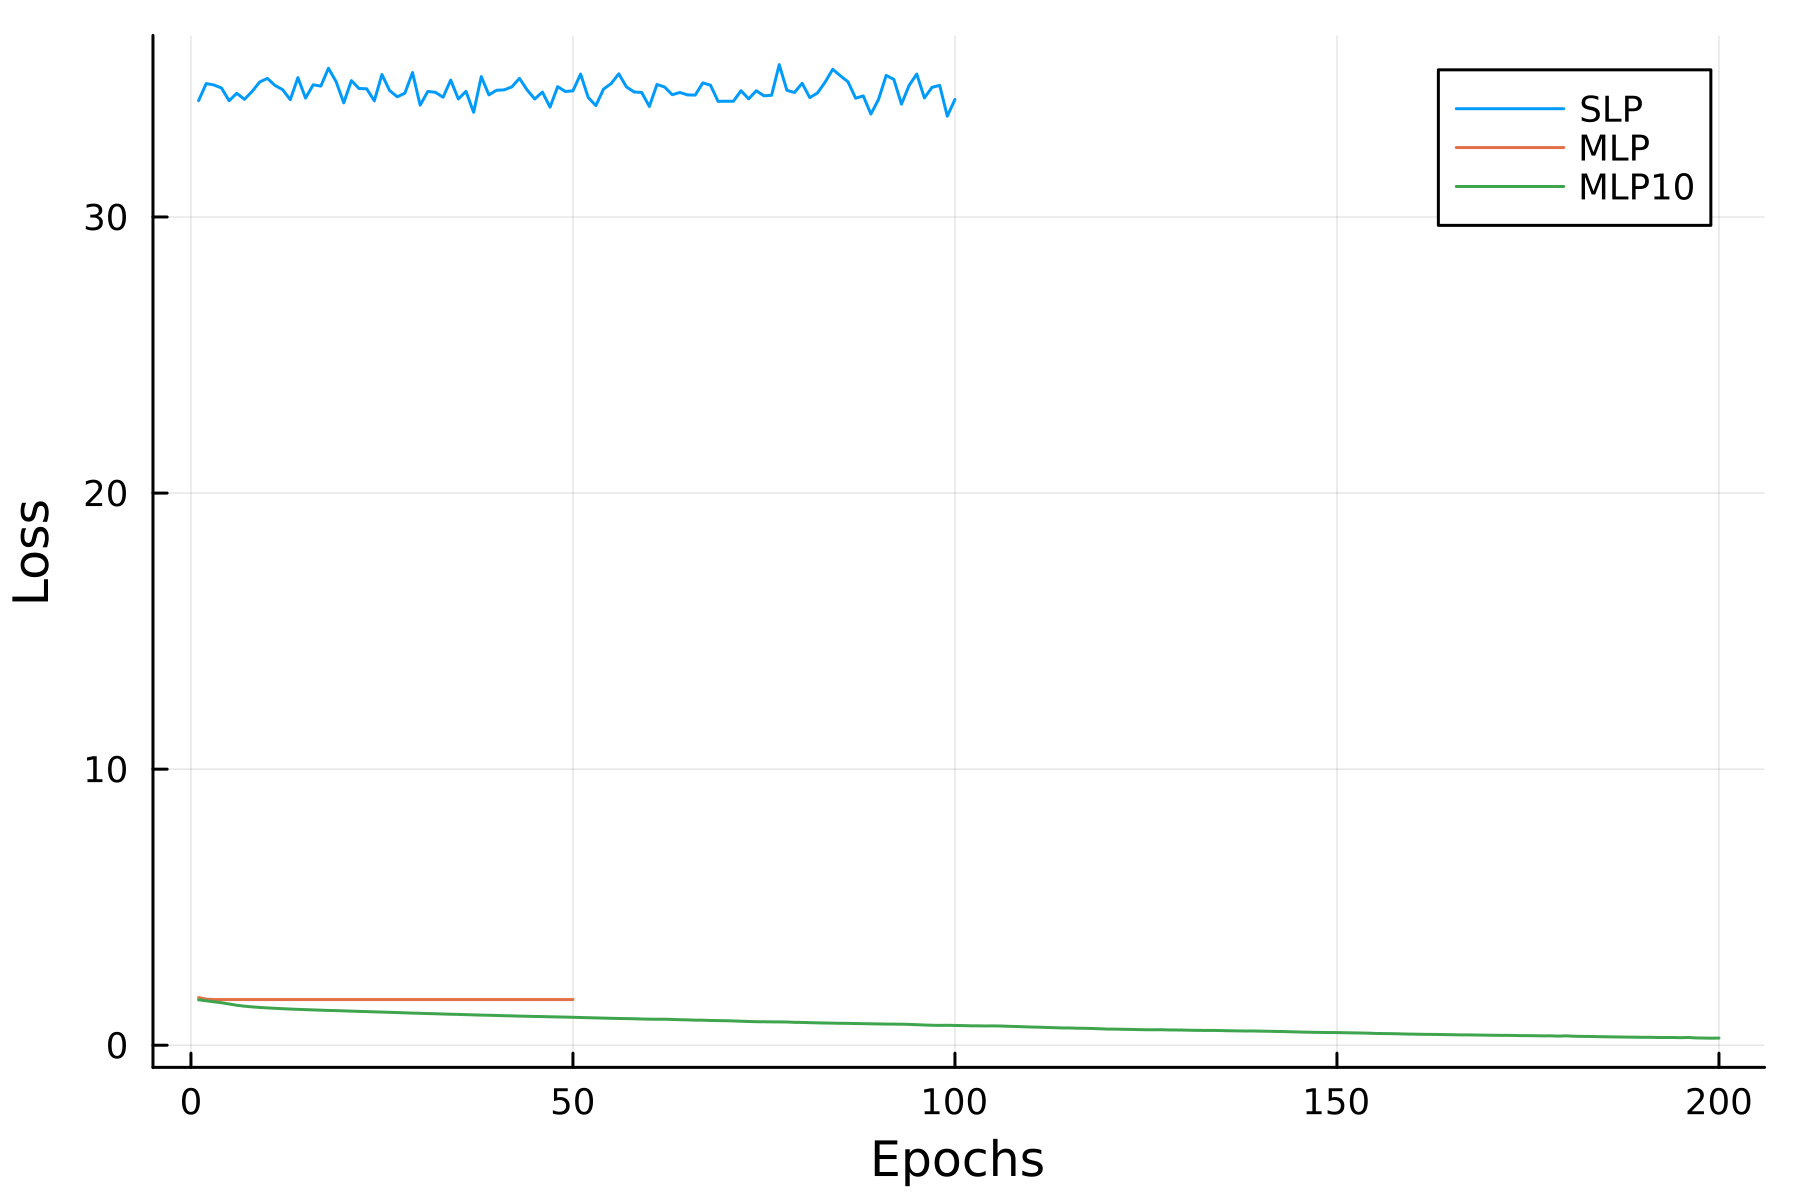
\includegraphics[width=\textwidth]{loss_plot_25_8}
        \caption{Training losses}
        \label{fig:loss}
    \end{subfigure}
    \end{minipage}
    \\
    \centering
    \begin{minipage}[b]{.6\textwidth}
    \begin{subfigure}[b]{\textwidth}
        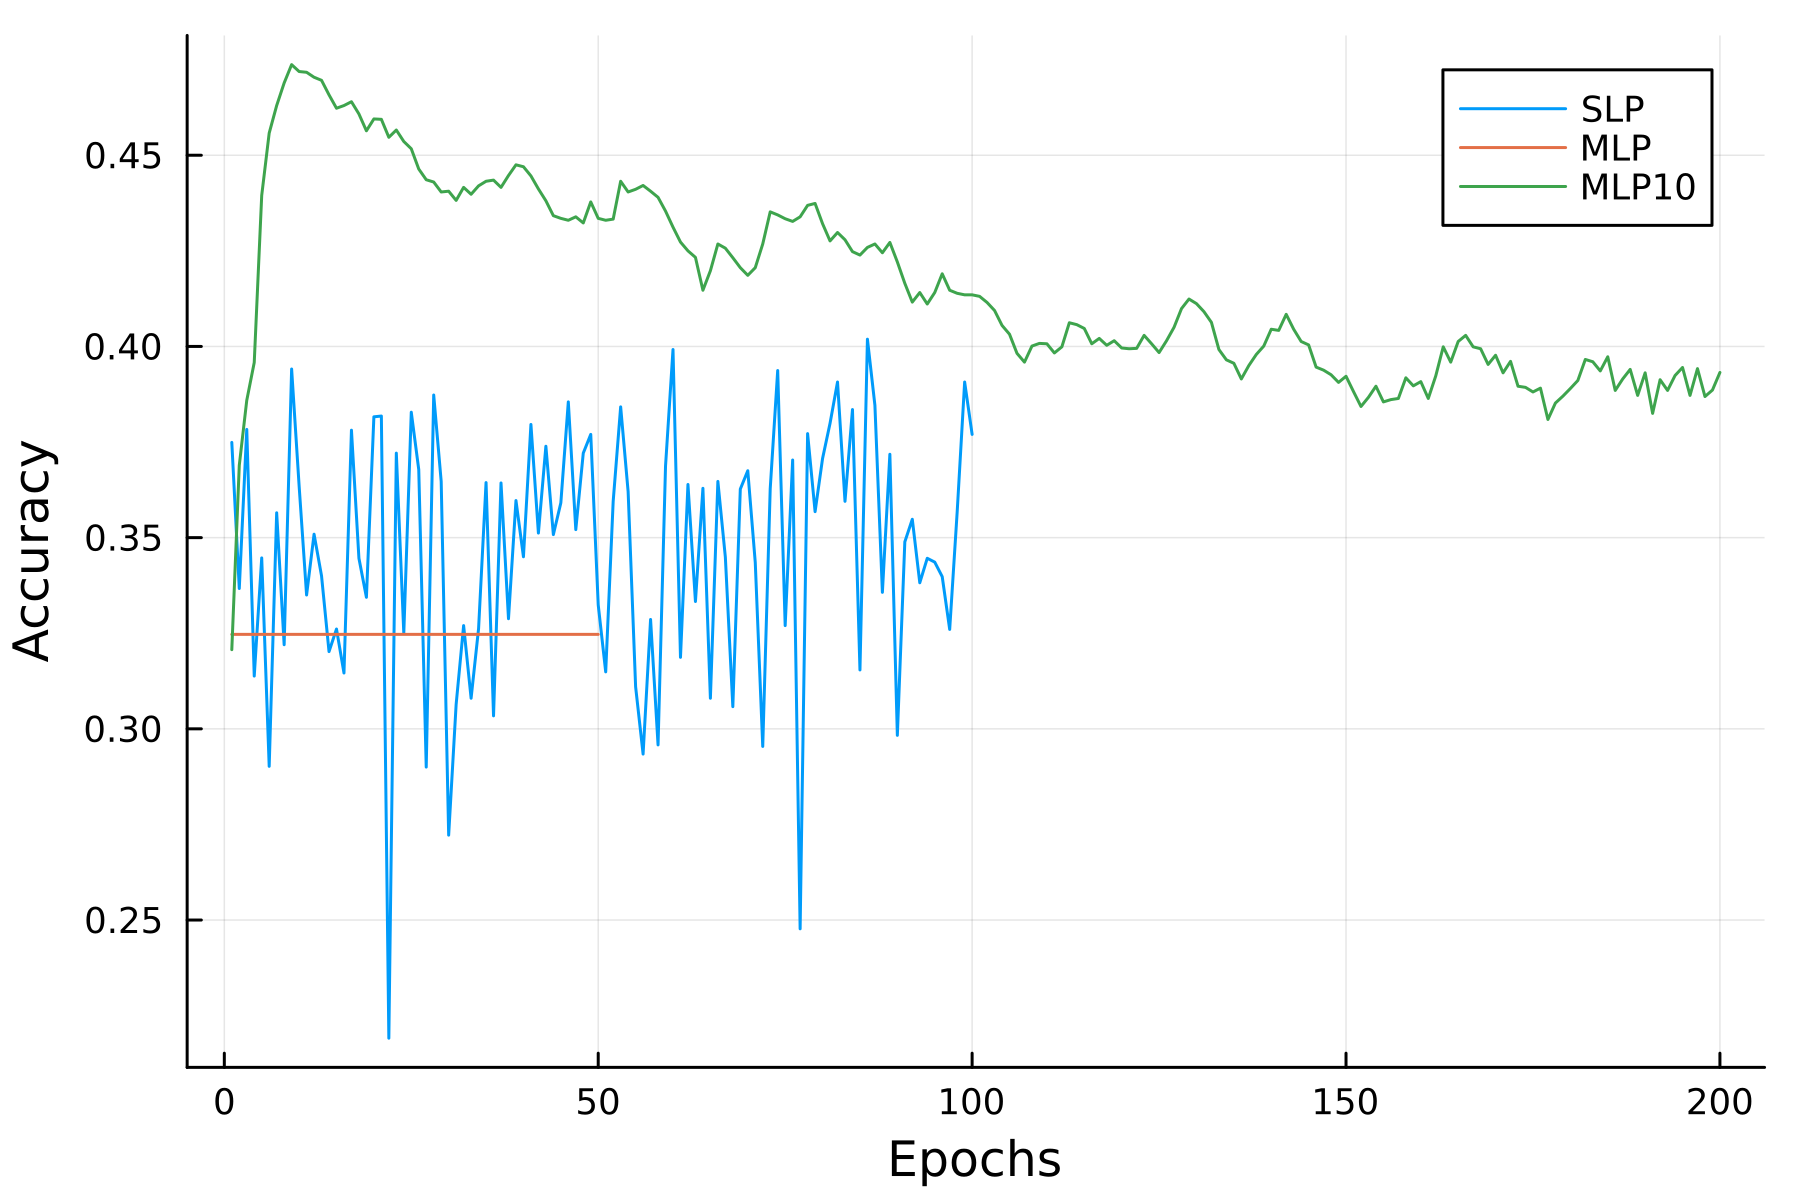
\includegraphics[width=\textwidth]{accuracy_plot_25_8}
        \caption{Accuracies}
        \label{fig:accuracy}
    \end{subfigure}
    \end{minipage}
    \\
    \centering
    \begin{minipage}[b]{.6\textwidth}
    \begin{subfigure}[b]{\textwidth}
        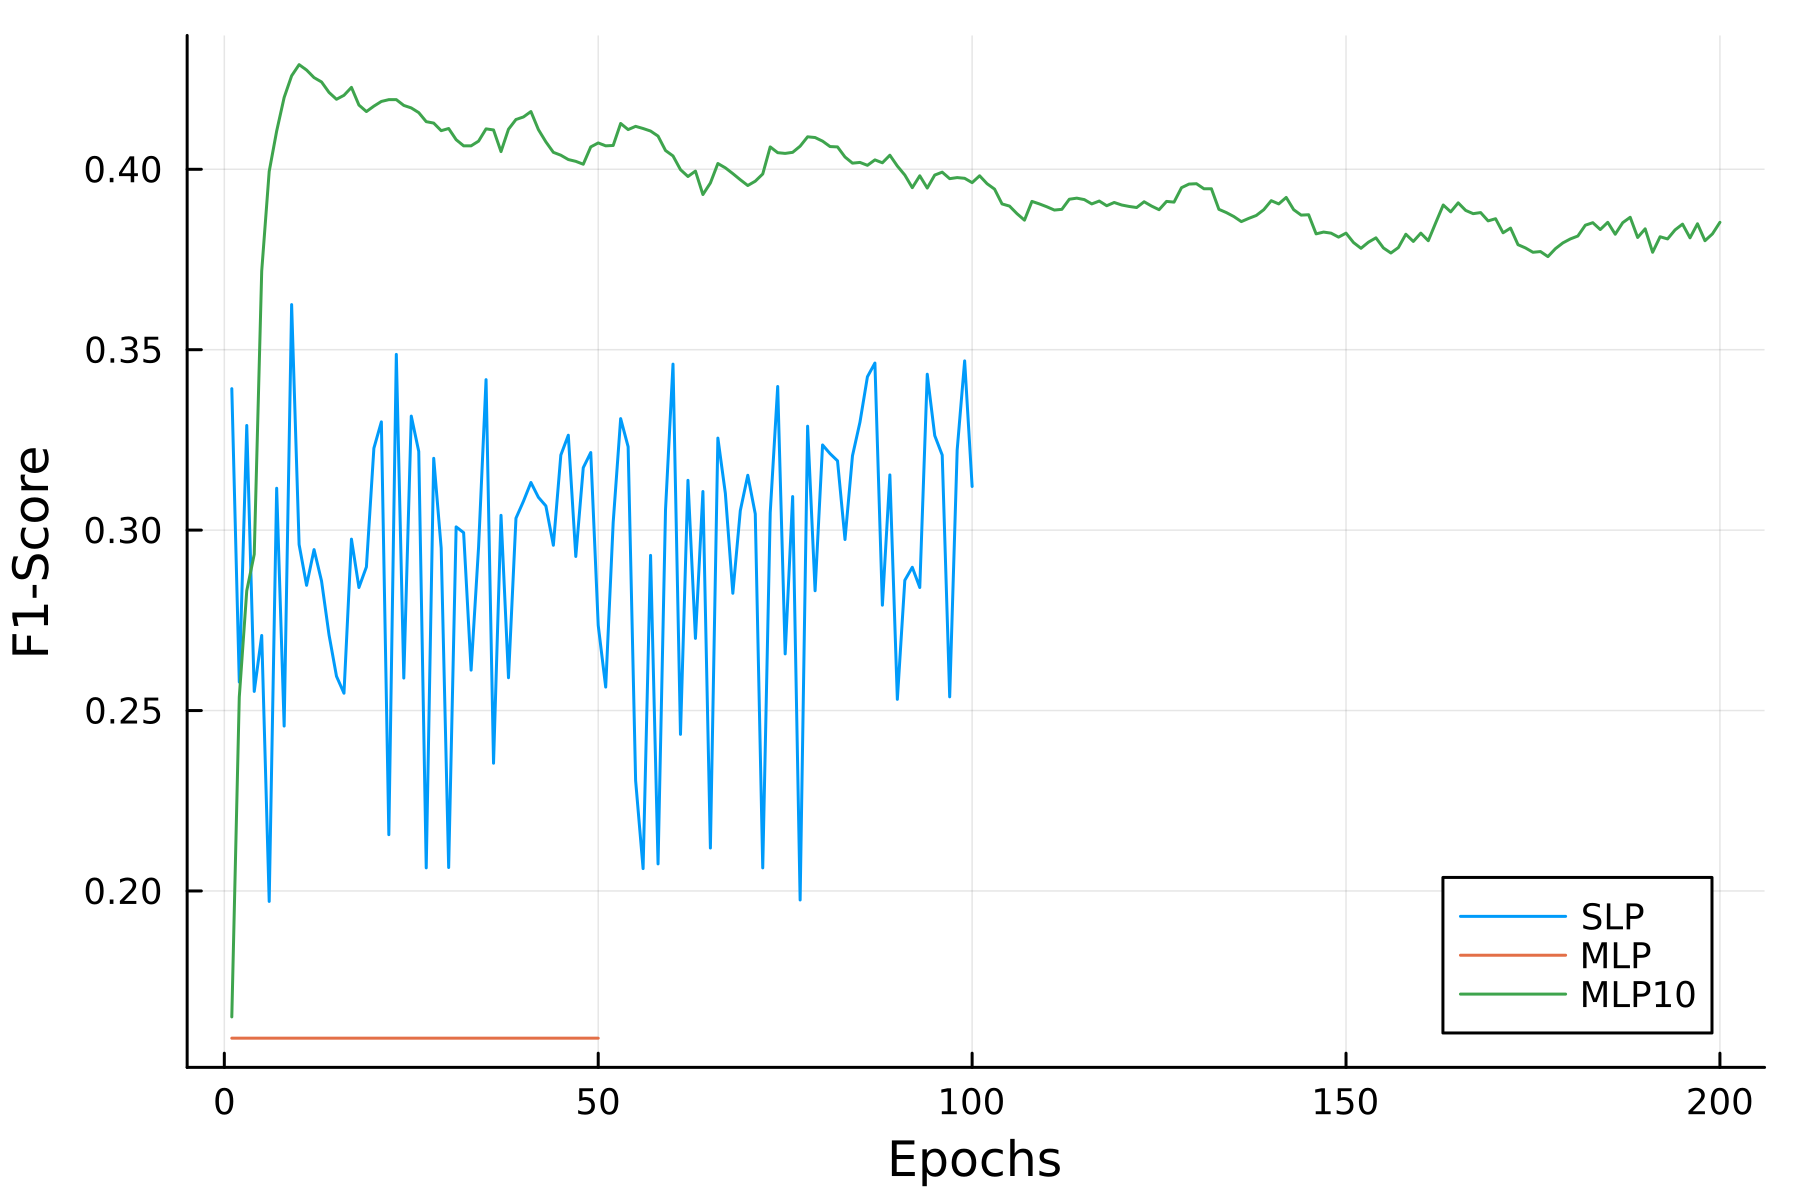
\includegraphics[width=\textwidth]{f1_plot_25_8}
        \caption{F1-scores}\label{fig:f1}
    \end{subfigure}
    \end{minipage}
    \caption{(a) cross-entropy losses (b) accuracies (c) F1-scores of all perceptron-based configurations tested. Trained with neighborhood-encodings of 60 \% of the training dataset of NetSurfP 2.0. Here $n=25$ and the secondary structure classification is dssp8-based. Note that the SLP and 1-layer MLP model was evaluated using fewer epochs than their 10-layer counterpart.}\label{fig:she2}
    \end{figure}

\begin{figure}[H]
        \centering
        \begin{minipage}[b]{.6\textwidth}
            \begin{subfigure}[b]{\textwidth}
            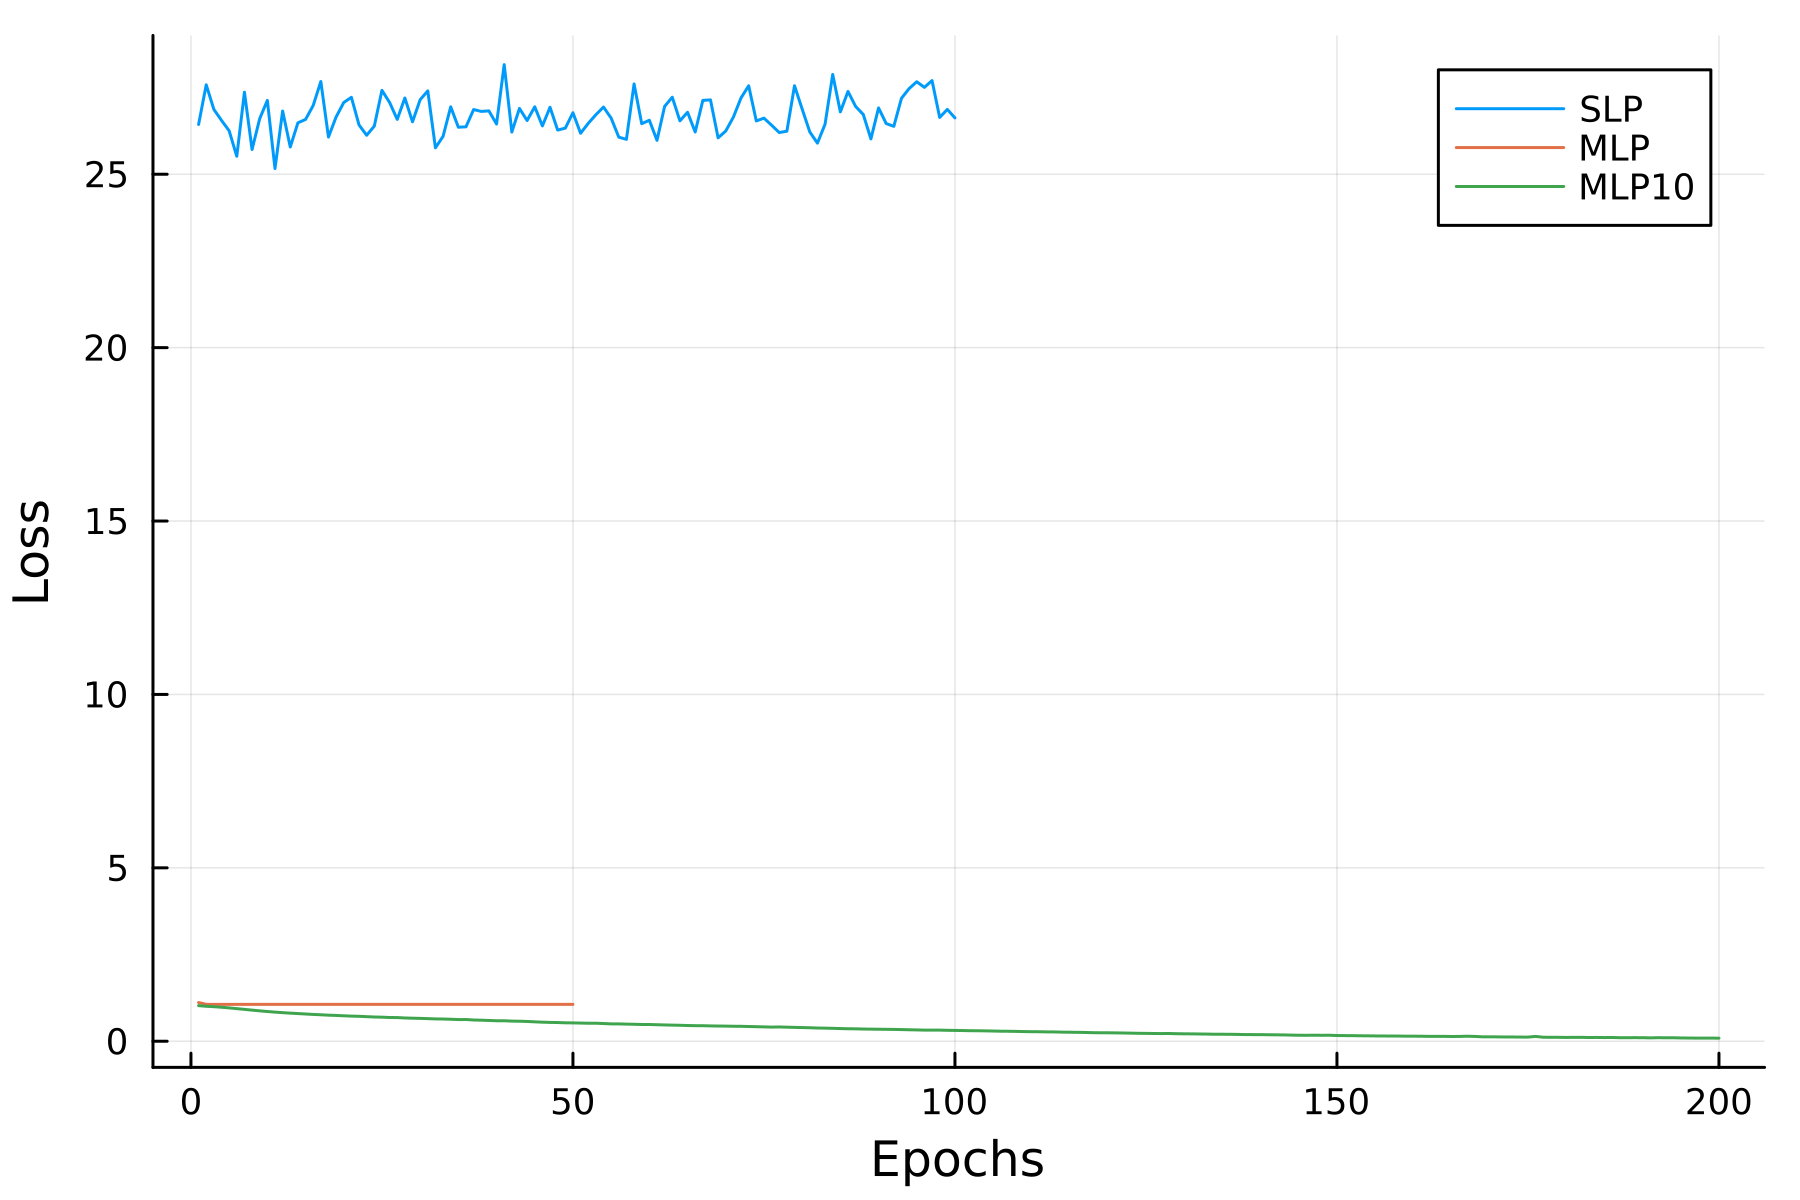
\includegraphics[width=\textwidth]{loss_plot_100_3}
            \caption{Training losses}
            \label{fig:loss}
        \end{subfigure}
        \end{minipage}
        \\
        \centering
        \begin{minipage}[b]{.6\textwidth}
        \begin{subfigure}[b]{\textwidth}
            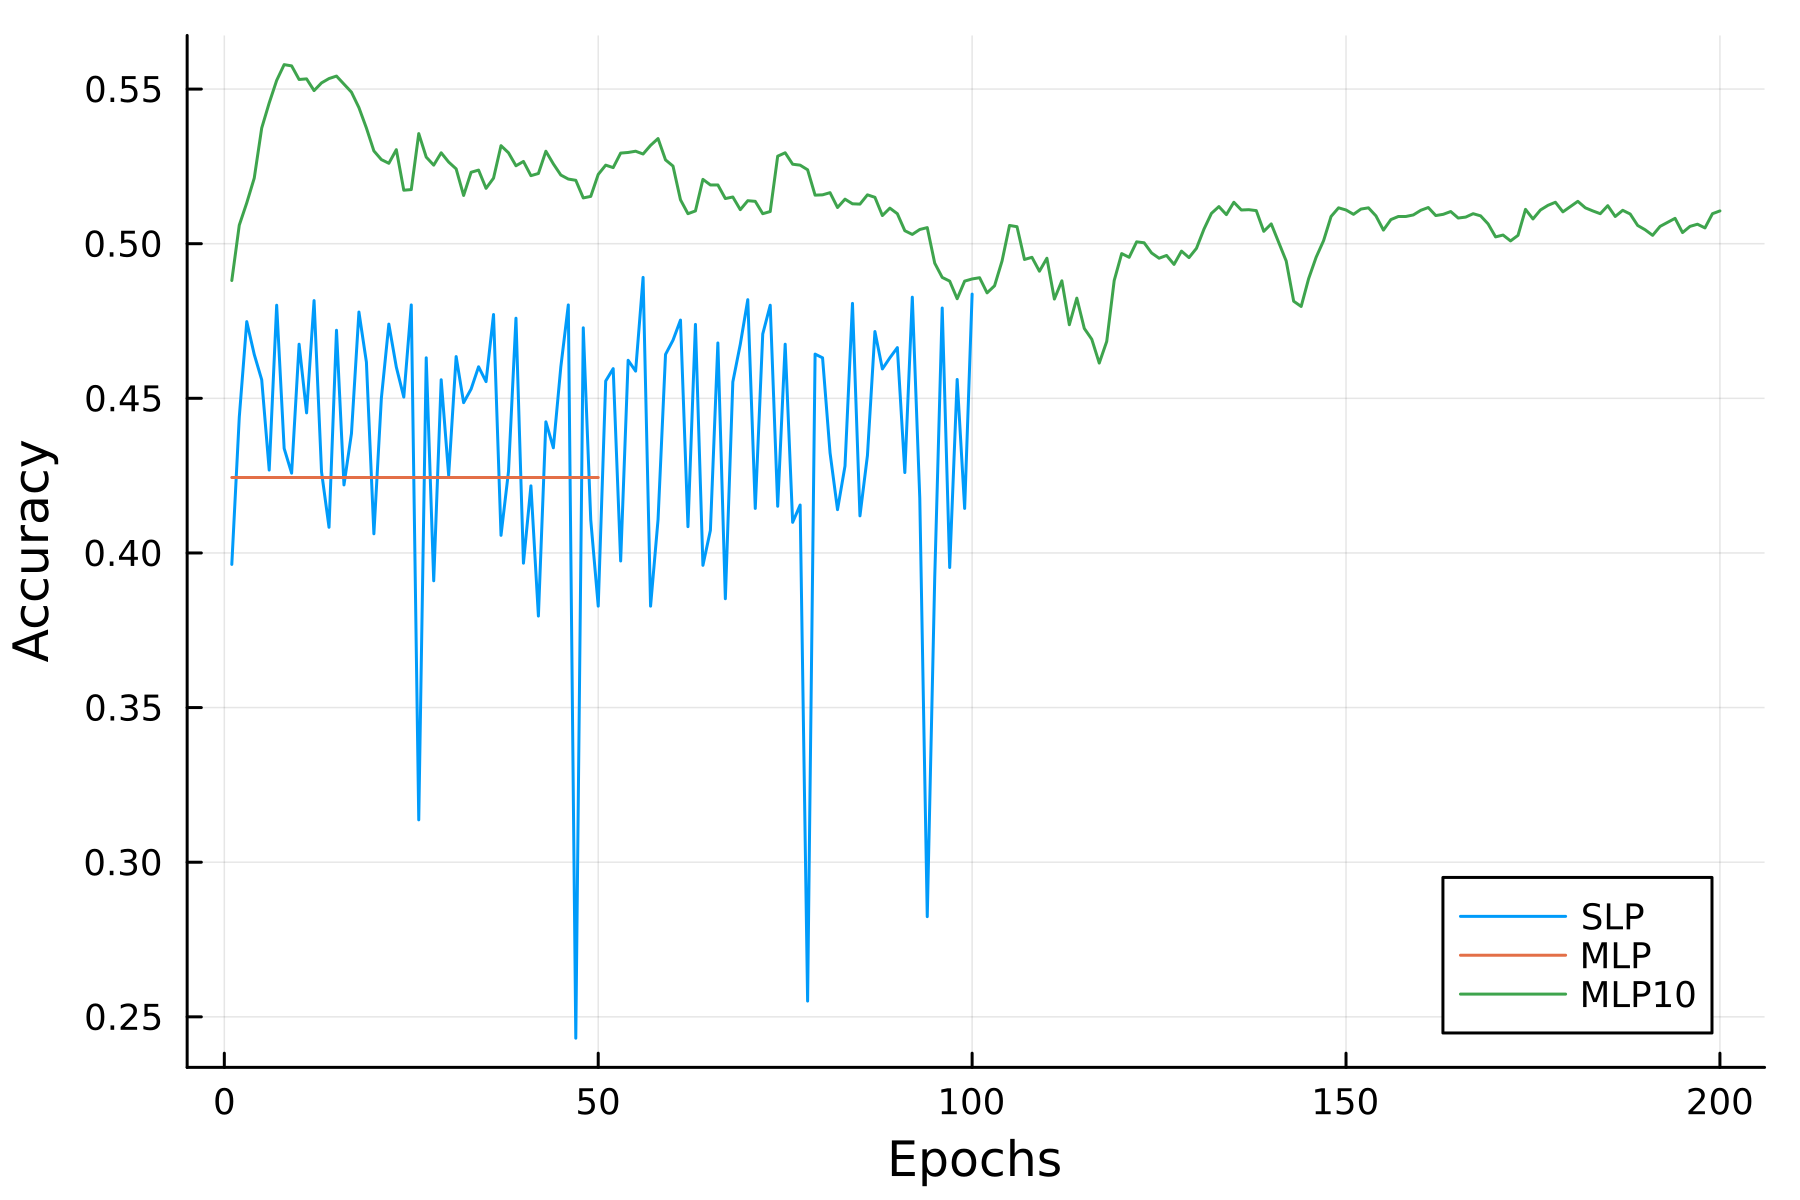
\includegraphics[width=\textwidth]{accuracy_plot_100_3}
            \caption{Accuracies}
            \label{fig:accuracy}
        \end{subfigure}
        \end{minipage}
        \\
        \centering
        \begin{minipage}[b]{.6\textwidth}
        \begin{subfigure}[b]{\textwidth}
            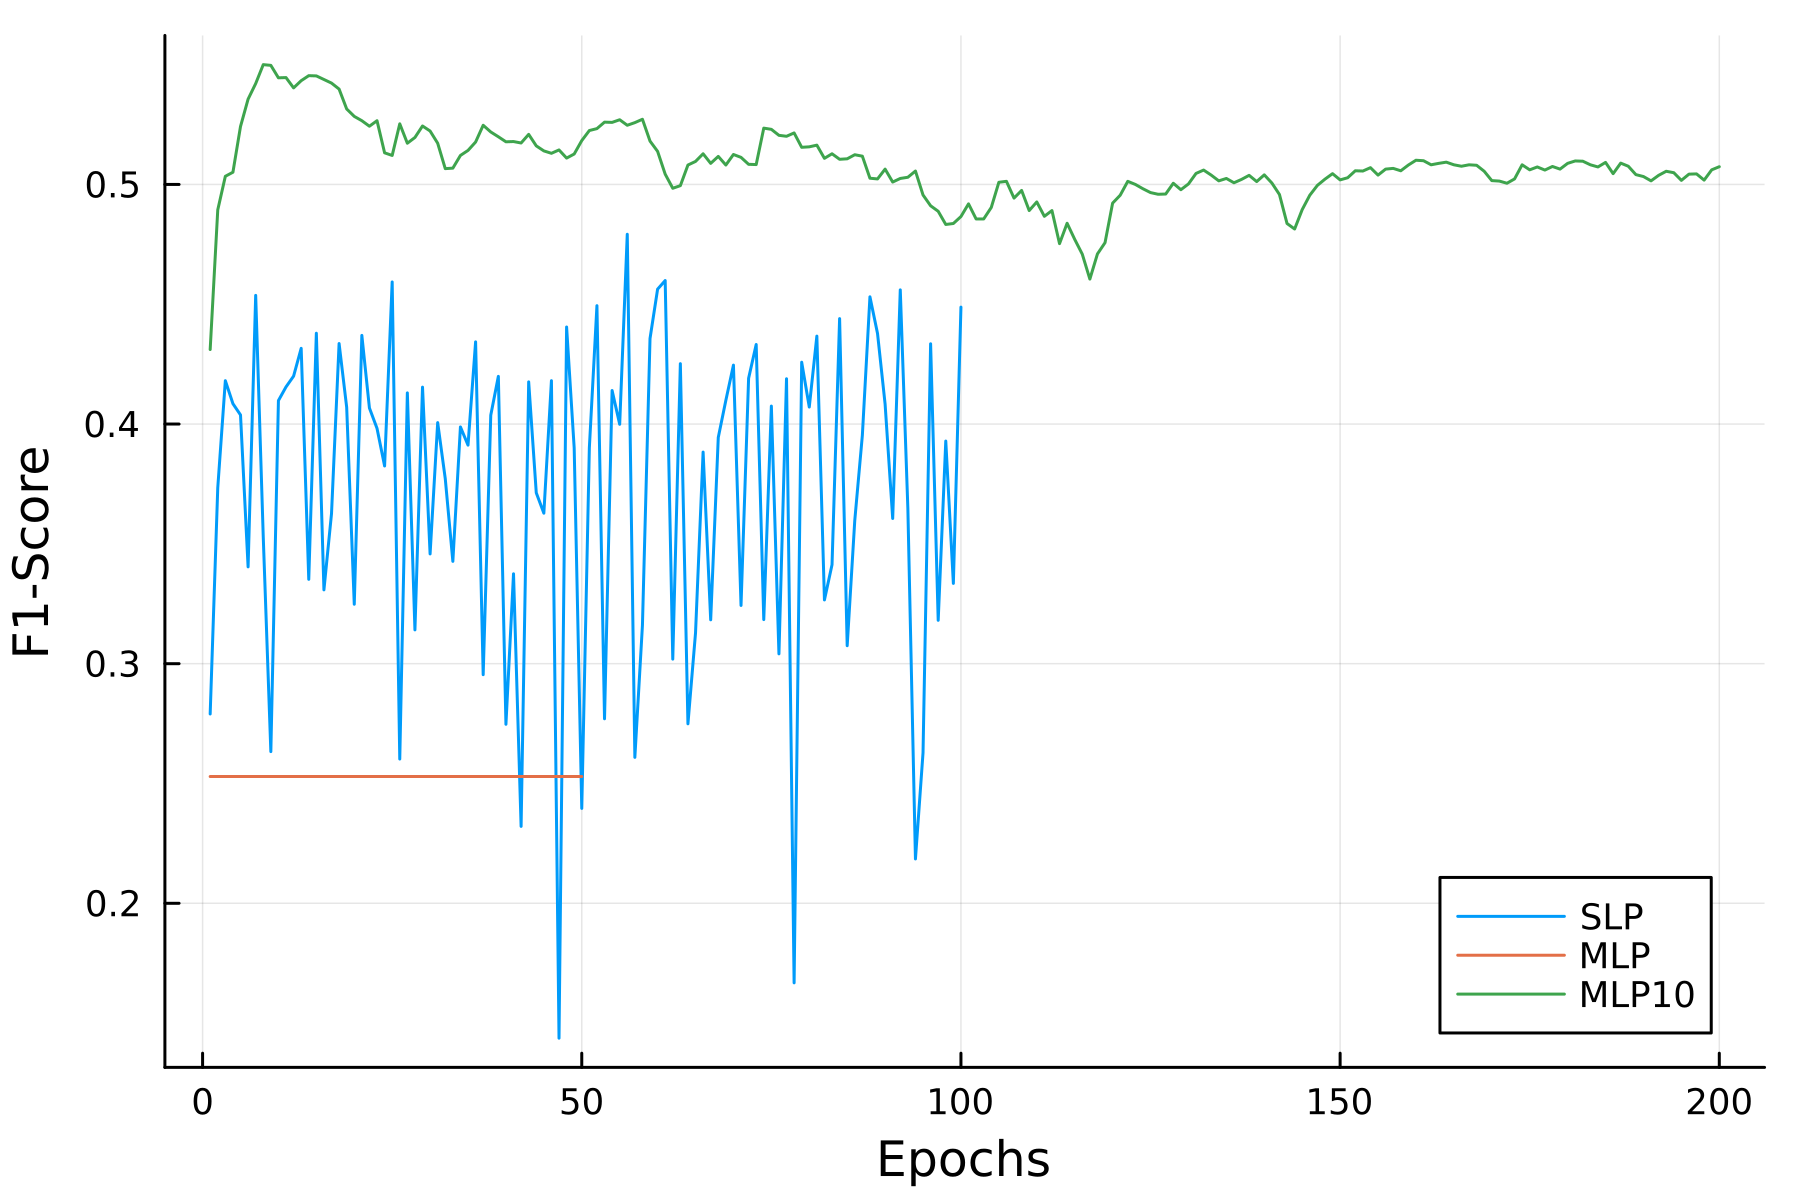
\includegraphics[width=\textwidth]{f1_plot_100_3}
            \caption{F1-scores}\label{fig:f1}
        \end{subfigure}
        \end{minipage}
        \caption{(a) cross-entropy losses (b) accuracies (c) F1-scores of all perceptron-based configurations tested. Trained with neighborhood-encodings of 60 \% of the training dataset of NetSurfP 2.0. Here $n=100$ and the secondary structure classification is dssp3-based. Note that the SLP and 1-layer MLP model was evaluated using fewer epochs than their 10-layer counterpart.}\label{fig:she3}
        \end{figure}

        \begin{figure}[H]
            \centering
            \begin{minipage}[b]{.6\textwidth}
                \begin{subfigure}[b]{\textwidth}
                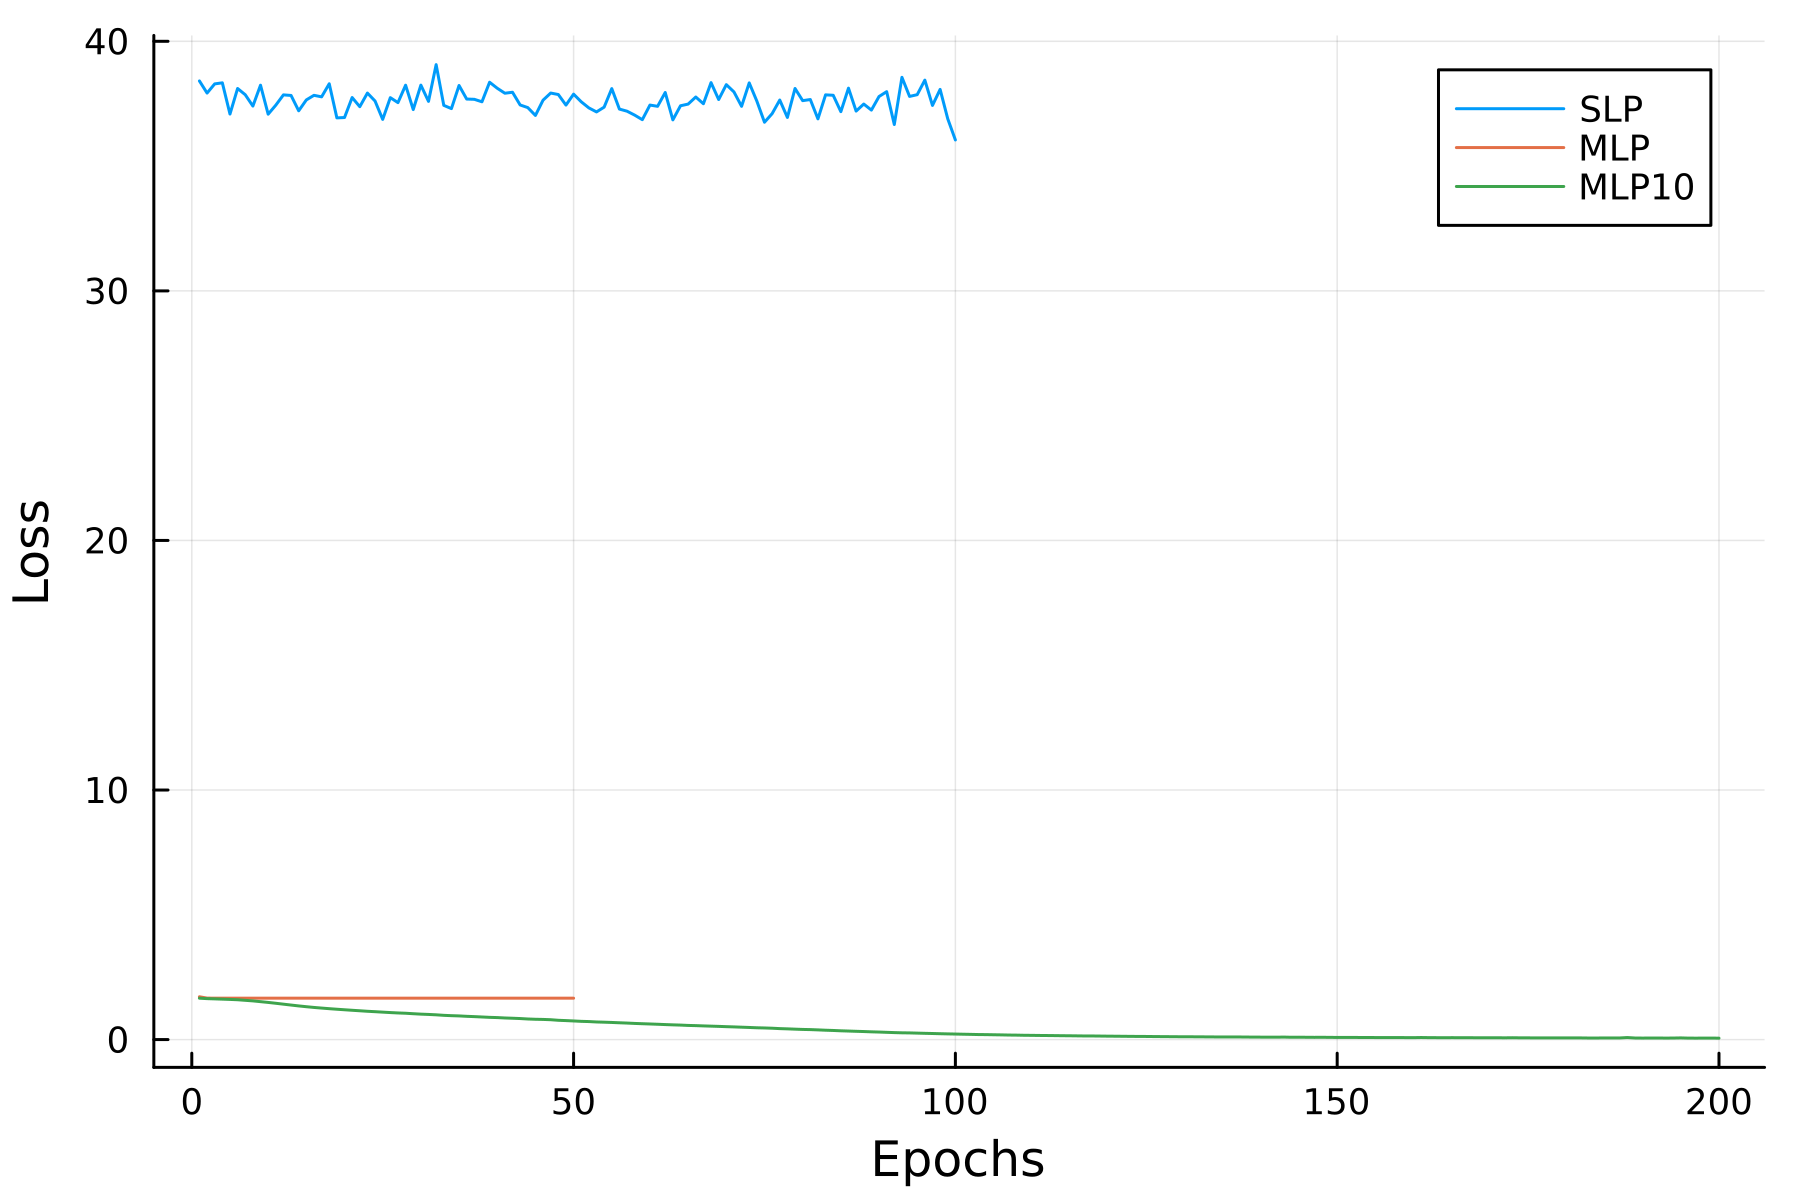
\includegraphics[width=\textwidth]{loss_plot_100_8}
                \caption{Training losses}
                \label{fig:loss}
            \end{subfigure}
            \end{minipage}
            \\
            \centering
            \begin{minipage}[b]{.6\textwidth}
            \begin{subfigure}[b]{\textwidth}
                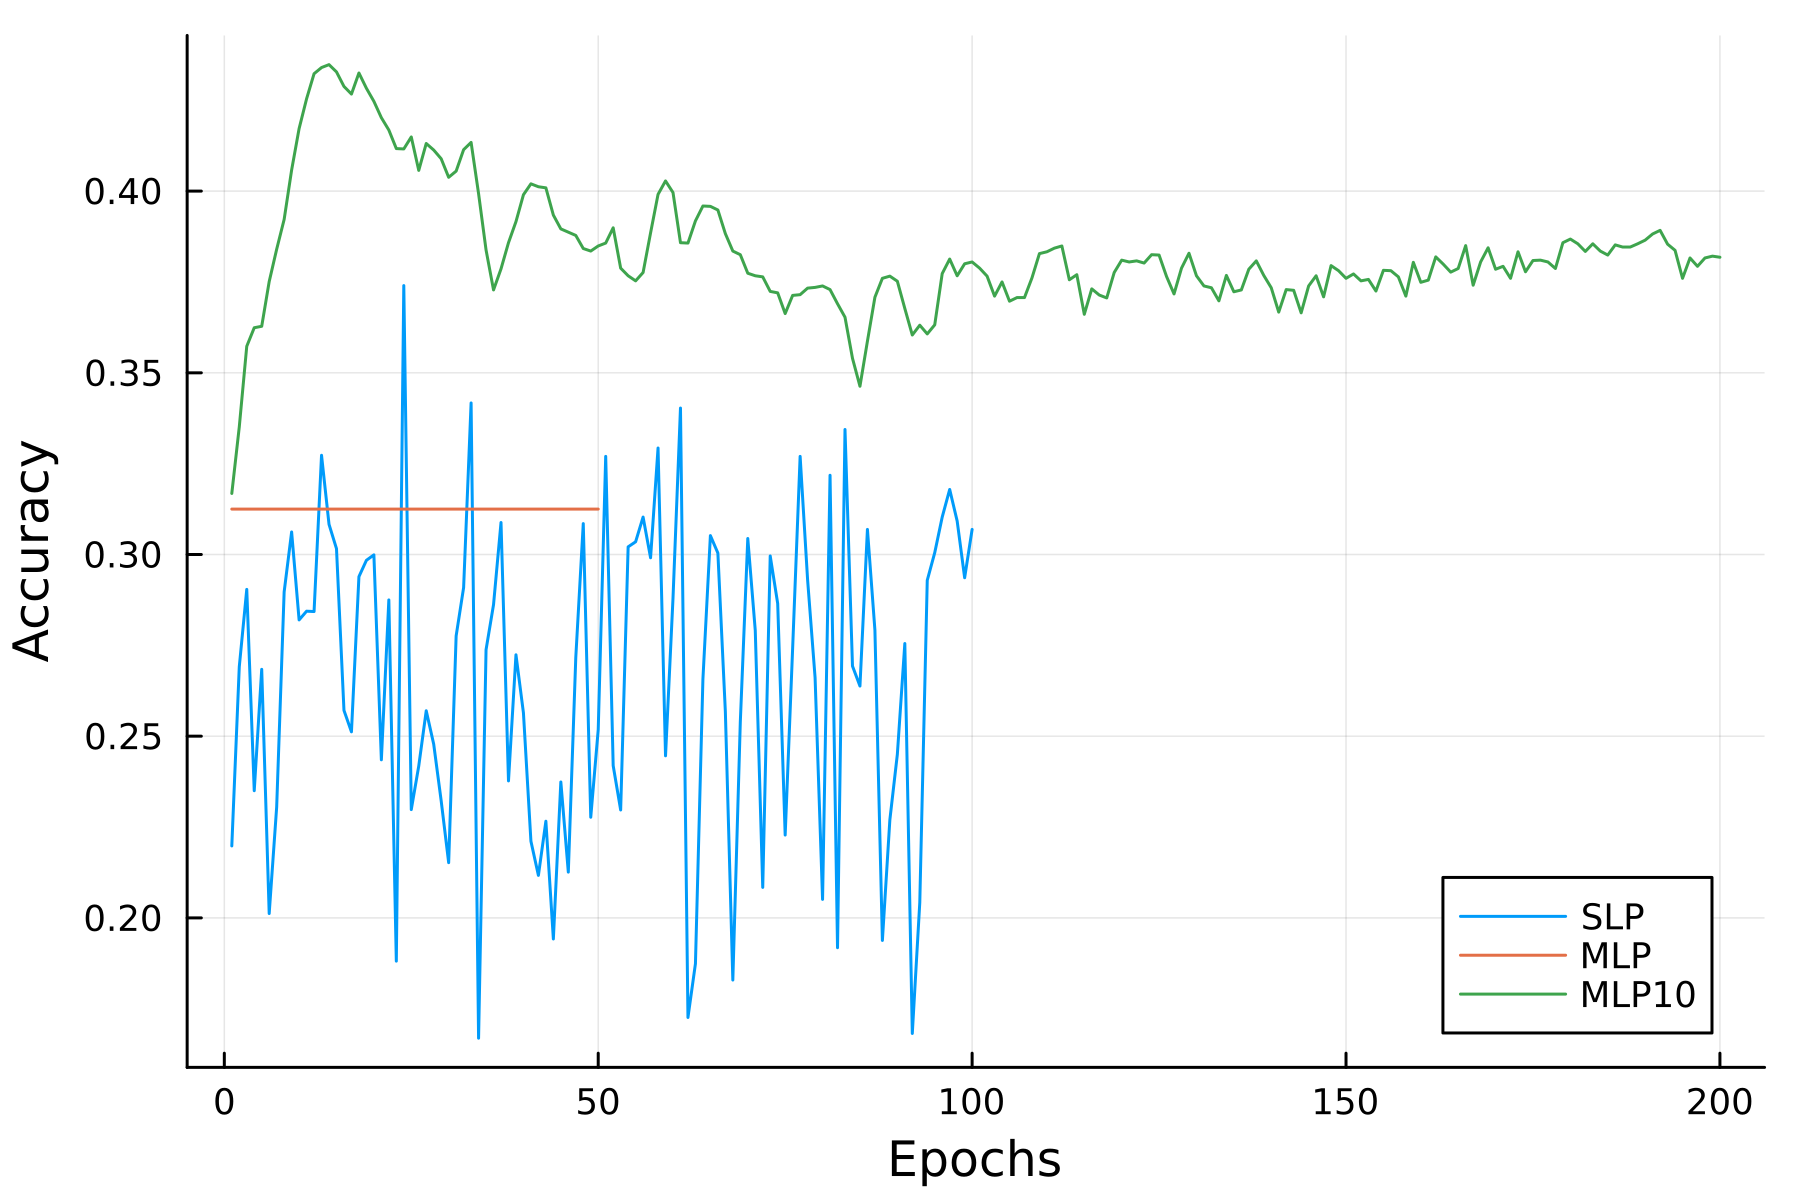
\includegraphics[width=\textwidth]{accuracy_plot_100_8}
                \caption{Accuracies}
                \label{fig:accuracy}
            \end{subfigure}
            \end{minipage}
            \\
            \centering
            \begin{minipage}[b]{.6\textwidth}
            \begin{subfigure}[b]{\textwidth}
                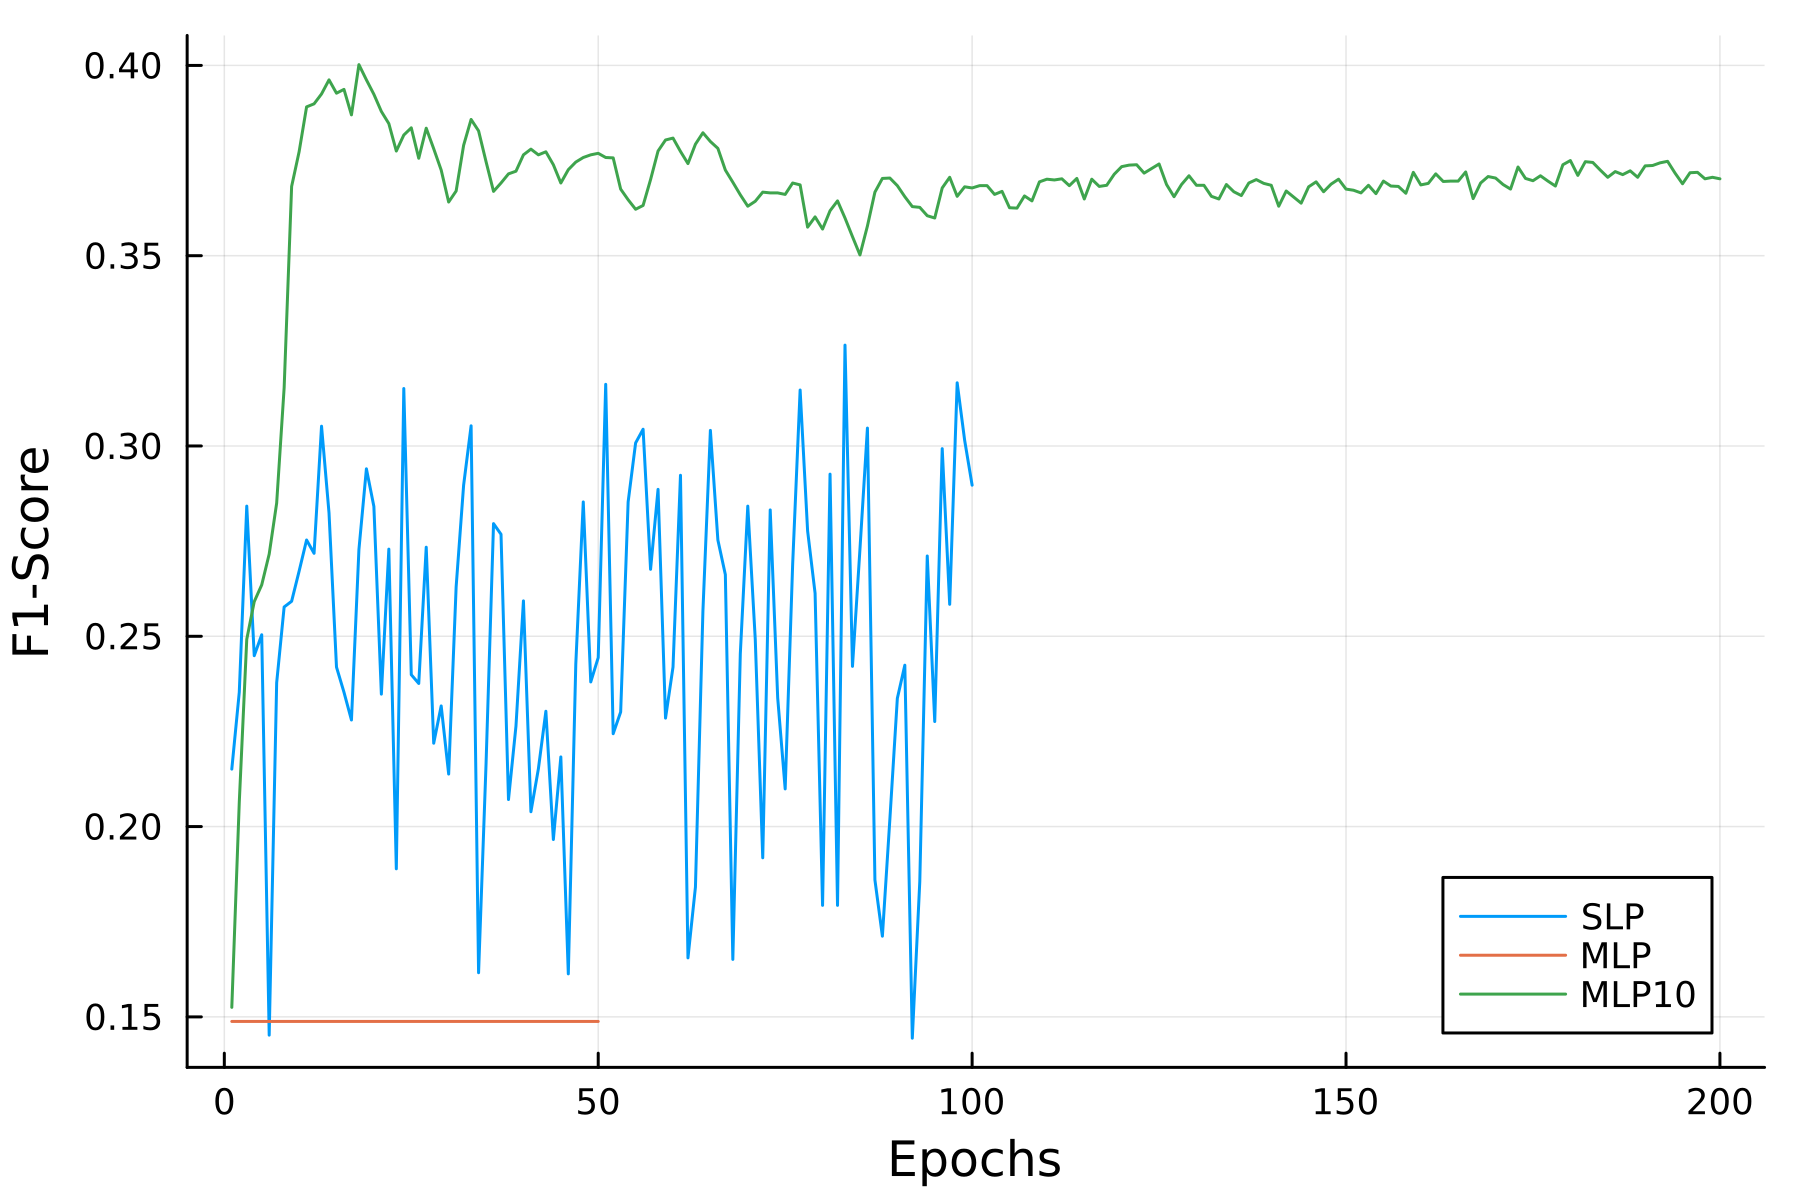
\includegraphics[width=\textwidth]{f1_plot_100_8}
                \caption{F1-scores}\label{fig:f1}
            \end{subfigure}
            \end{minipage}
            \caption{(a) cross-entropy losses (b) accuracies (c) F1-scores of all perceptron-based configurations tested. Trained with neighborhood-encodings of 60 \% of the training dataset of NetSurfP 2.0. Here $n=100$ and the secondary structure classification is dssp8-based. Note that the SLP and 1-layer MLP model was evaluated using fewer epochs than their 10-layer counterpart.}\label{fig:she4}
            \end{figure}

\end{appendices}

\end{document}
